\section{Results}

The possible implementation of the CLaRyS Compton camera as a monitoring system for ion beam therapy has been investigated. 
%The detection efficiency of the camera has been estimated with point-like gamma sources, and the relative efficiency in detecting various kinds of coincidence events has been studied. 
%Events with a single scatterer layer hit have been selected for the following part of the analysis (from section~\ref{Results::efficiency}), for the sake of simplicity and given the results of this preliminary investigation. This choice is made as a first approach for the feasibility study, and the obtained results can be considered as the minimal camera performance, and are expected to be improved by the inclusion of other kind of events. 
%The camera absolute efficiency has been estimated as a function of the gamma energy and with the point-like sources set in different positions with respect to the center of the camera, with and without the application of detection energy thresholds. 
The camera has been exposed to point-like gamma sources to study the detection efficiency.
A PMMA cylindrical phantom has been simulated and exposed to proton and carbon beams at increasing intensities for an analysis of the prompt gamma detection environment (background, random coincidence contamination). The camera precision in the identification of the fall-off of the prompt gamma emission profile has been investigated. 
%For this purpose, the comparison of two different reconstruction methods (line-cone analytical reconstruction and MLEM iterative algorithm) is presented. 
In the following sections we show the obtained results. 


\subsection{Detection efficiency of various types of true coincidences}
\label{Results::relefficiency}
Figure~\ref{fig::eff_evKind} shows the Compton camera efficiency in detecting the kinds of coincidence events described in section~\ref{MatMeth::events}, as a function of the gamma energy in the prompt-gamma energy range (between 300~keV and 6~MeV). The results show how the single events, consisting in the coincidence between an energy deposit in a single scatterer layer and in one single absorber block, decreases at increasing energy, in favor of an increase in the number of electron escape events (consisting in one primary photon Compton interaction in one scatterer layer, at least one interaction of the Compton escaped recoil electron in a different scatterer layer, and one primary photon interaction in one single absorber block). At the maximum investigated primary gamma energy,  the amount of electron escape collected events is more than 35\%. However, the single events represent more than 60\% of the total amount of collected events in all the explored energy range, so that the results in the following paragraphs are focused on this kind of events (with the other kinds of events rejected at the analysis stage), as first approach for a feasibility study. The amount of 3 or more photon-interaction events is limited and negligible over the whole energy range.

\begin{figure} [!hbtp]	
\centering
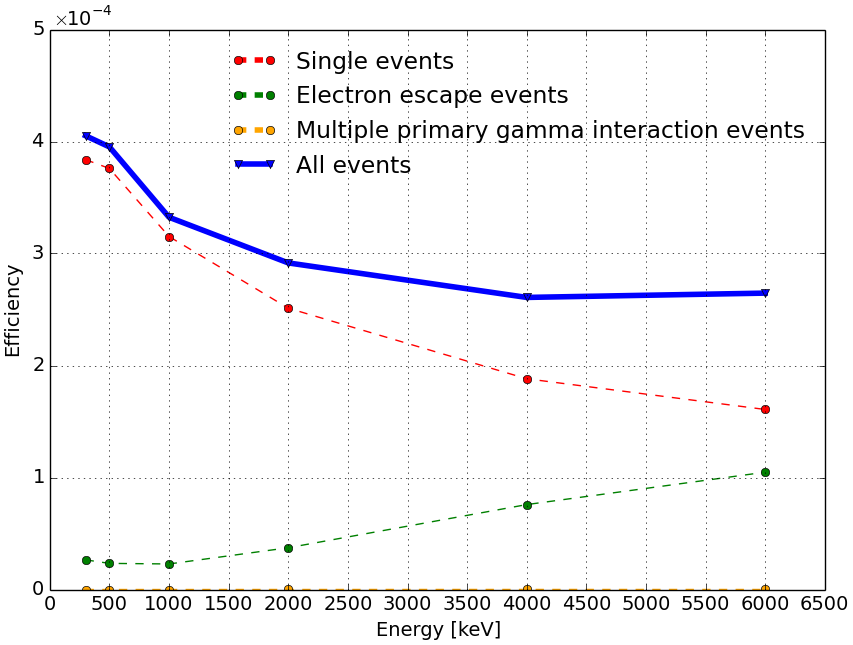
\includegraphics[width=0.6\textwidth]{./Figure/new/effVSenergy_trigger.png}
\caption{Compton camera efficiency as a function of the gamma energy for the different kind of possible coincidence events (see section~\ref{MatMeth::events}), as a function of the gamma energy.}
\label{fig::eff_evKind}
\end{figure}

\begin{figure} [!hbtp]	
\centering
%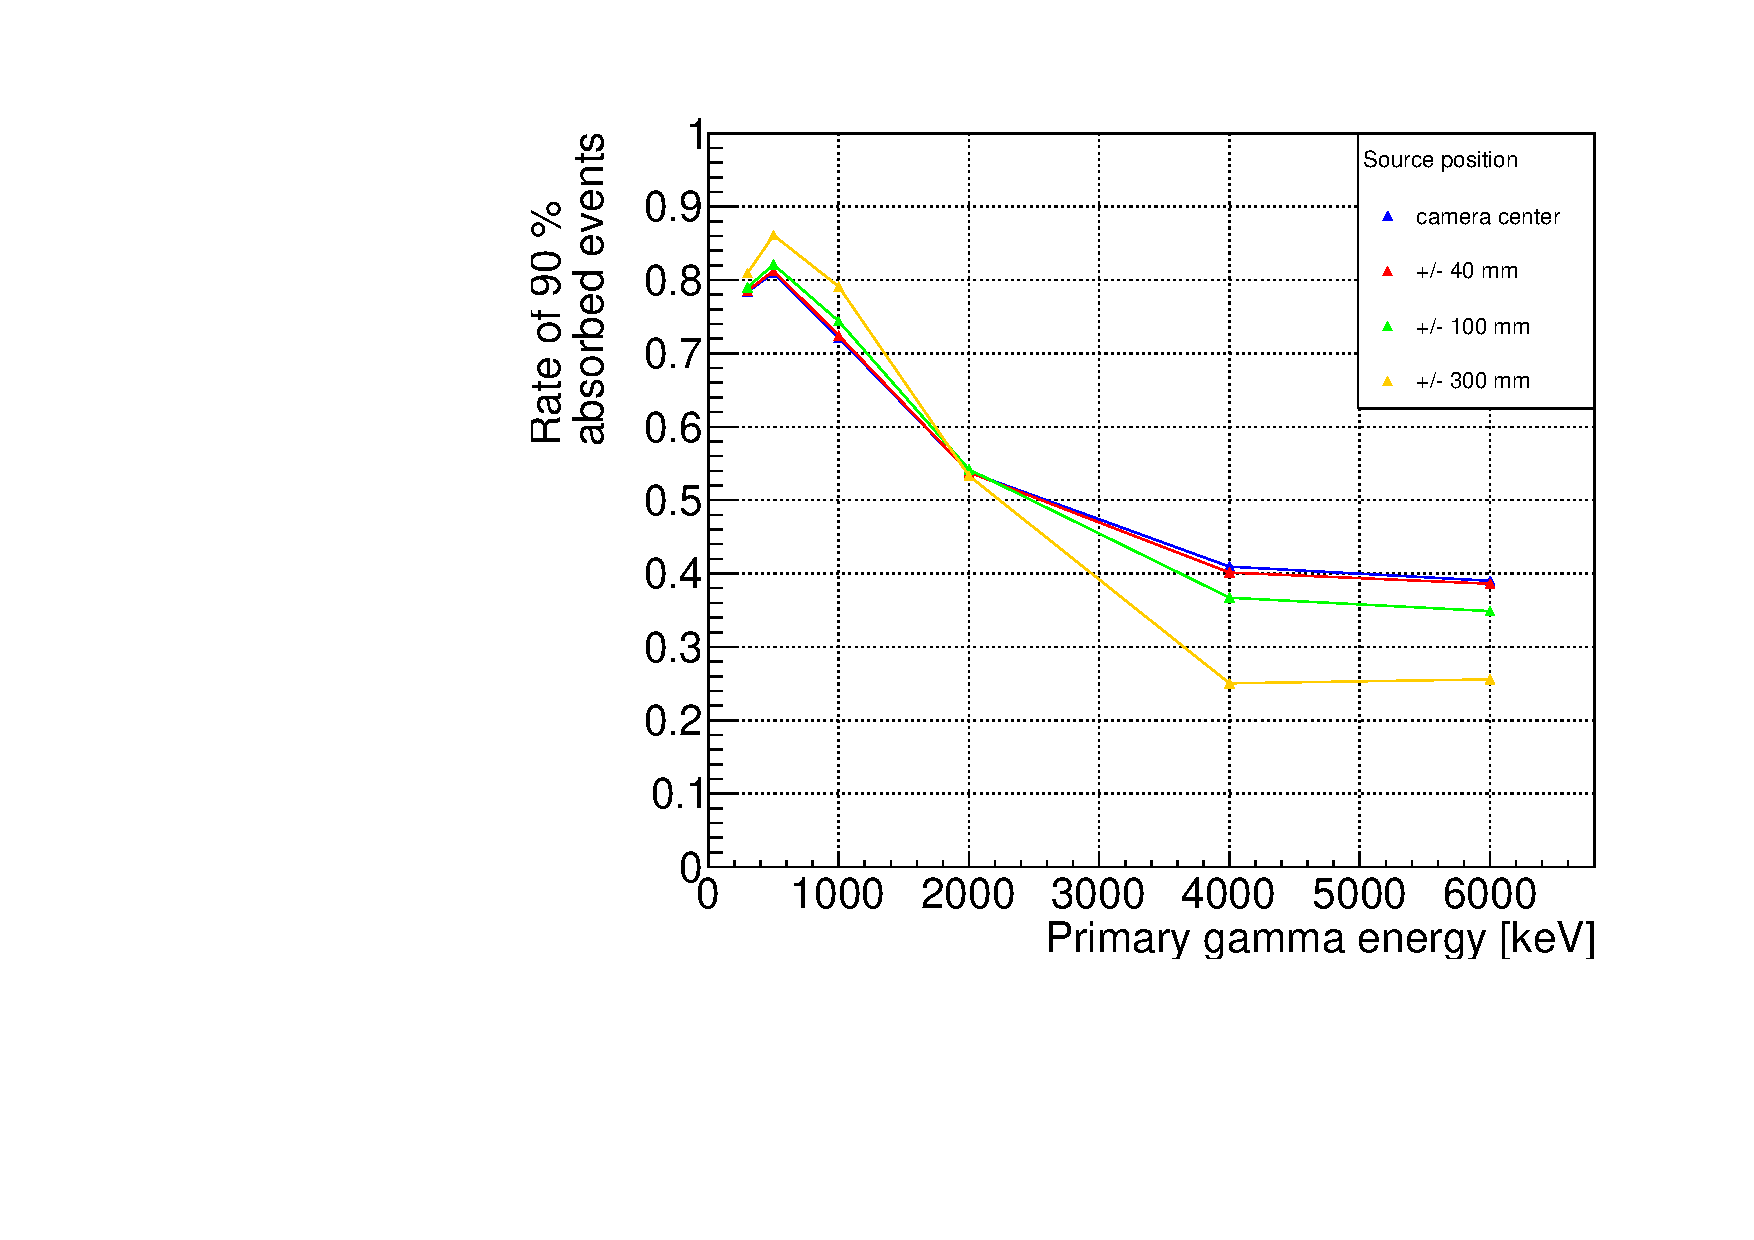
\includegraphics[width=0.7\textwidth]{./Figure/new/rate_90percent_energy_4distances.pdf}
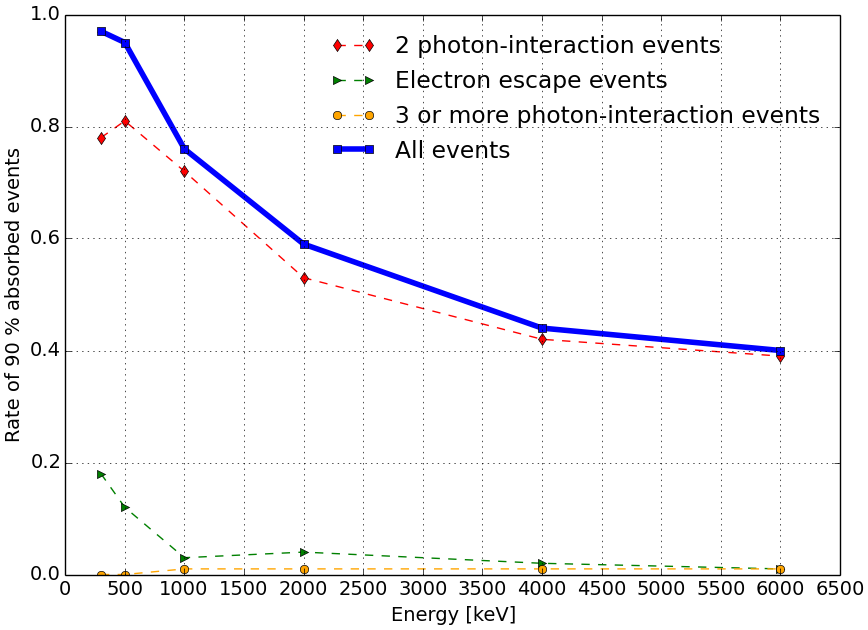
\includegraphics[width=0.6\textwidth]{./Figure/new/90absFracVSenergy_hadronth.png}
\caption{Ratio between coincidence events with more than 90\% of the primary photon energy absorbed in the detector layer and all detected coincidences as a function of the gamma energy. The curves shown the results for the different kind of possible coincidence events and for the all collected coincidences.}
\label{fig::rate_full_abs}
\end{figure}

Figure~\ref{fig::rate_full_abs} shows the rate of events with more than 90\% of the primary gamma energy deposited in the detector layers. The rate of 90\% absorbed events is reported for the different kinds of detected coincidences. As expected, the rate of almost fully absorbed events decreases as the energy increases, in a range between more than 80\% and 40\% for 300~keV and 6~MeV primary photon energy, respectively. The most of the 90\% absorbed events are single events, with the electron escape and multiple ones negligible for primary gamma energies above 1~MeV. At lower energy, the Compton recoil electron is often able to exit the scatterer layer where the Compton interaction takes place, but can be lost without further interactions, so that this kind of events is considered as single with an energy absorption below 90\%. This can explain the decrease of single almost full absorption at 300~keV. If the electron interacts with a scatterer layer, it is generally absorbed at low energy, explaining the increasing electron escape absorbed events below 1~MeV. 
As mentioned, these results led to the choice of limiting the further analysis (from section~\ref{Results::efficiency}) to events with a single scatterer layer involved, as first approach.
 
 \subsection{Absolute detection efficiency}
\label{Results::efficiency}
Figure~\ref{fig::efficiency_study} shows the absolute gamma detection efficiency as a function of the gamma source position with respect to the center of the camera in the transverse plane. On the left side, we show the results achieved without energy detection thresholds. On the right side realistic energy thresholds are applied on each detector section (50~keV for the scatterer layers and 100~keV for the absorber).

\begin{figure} [!hbtp]	
\centering
%\subfloat[]{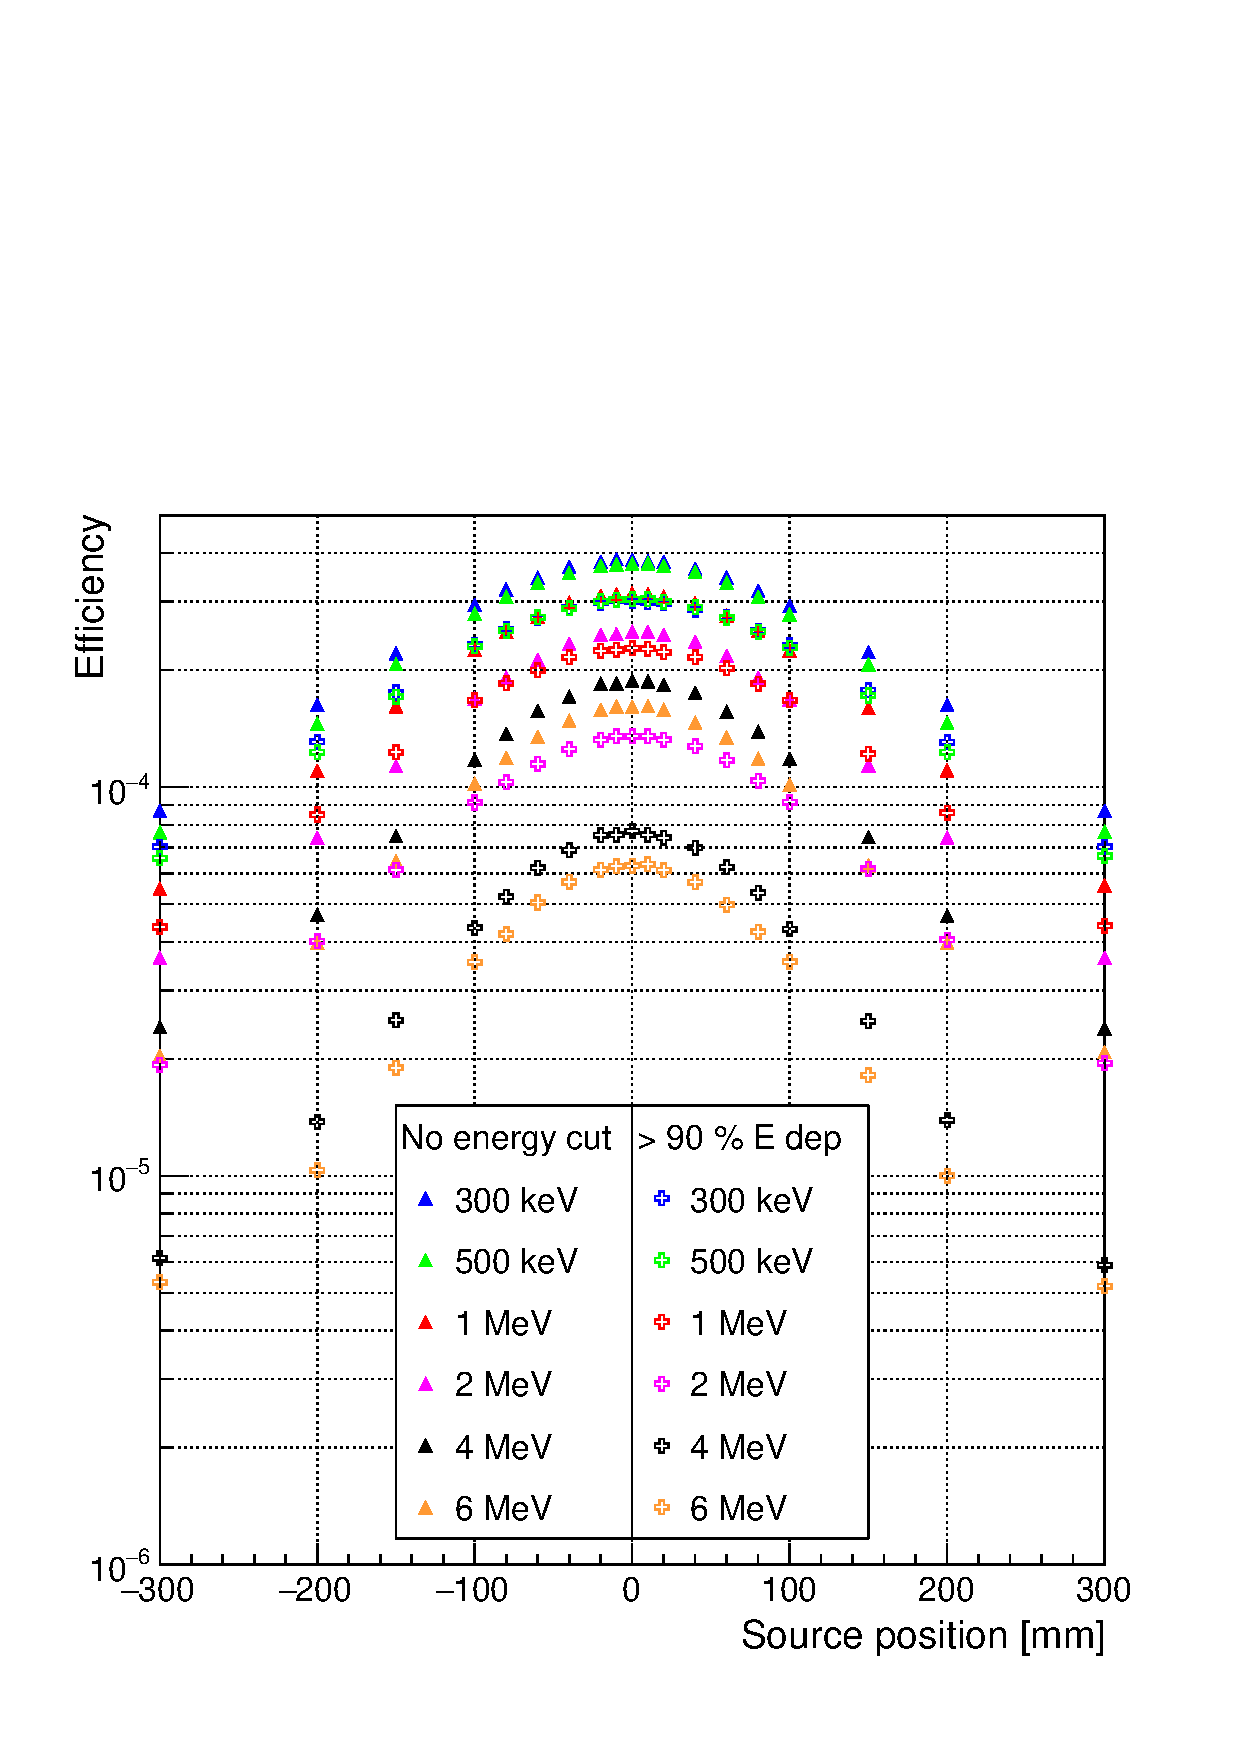
\includegraphics[width=0.5\textwidth]{./Figure/new/EffVSpos_withSumCut.pdf}}
\subfloat[]{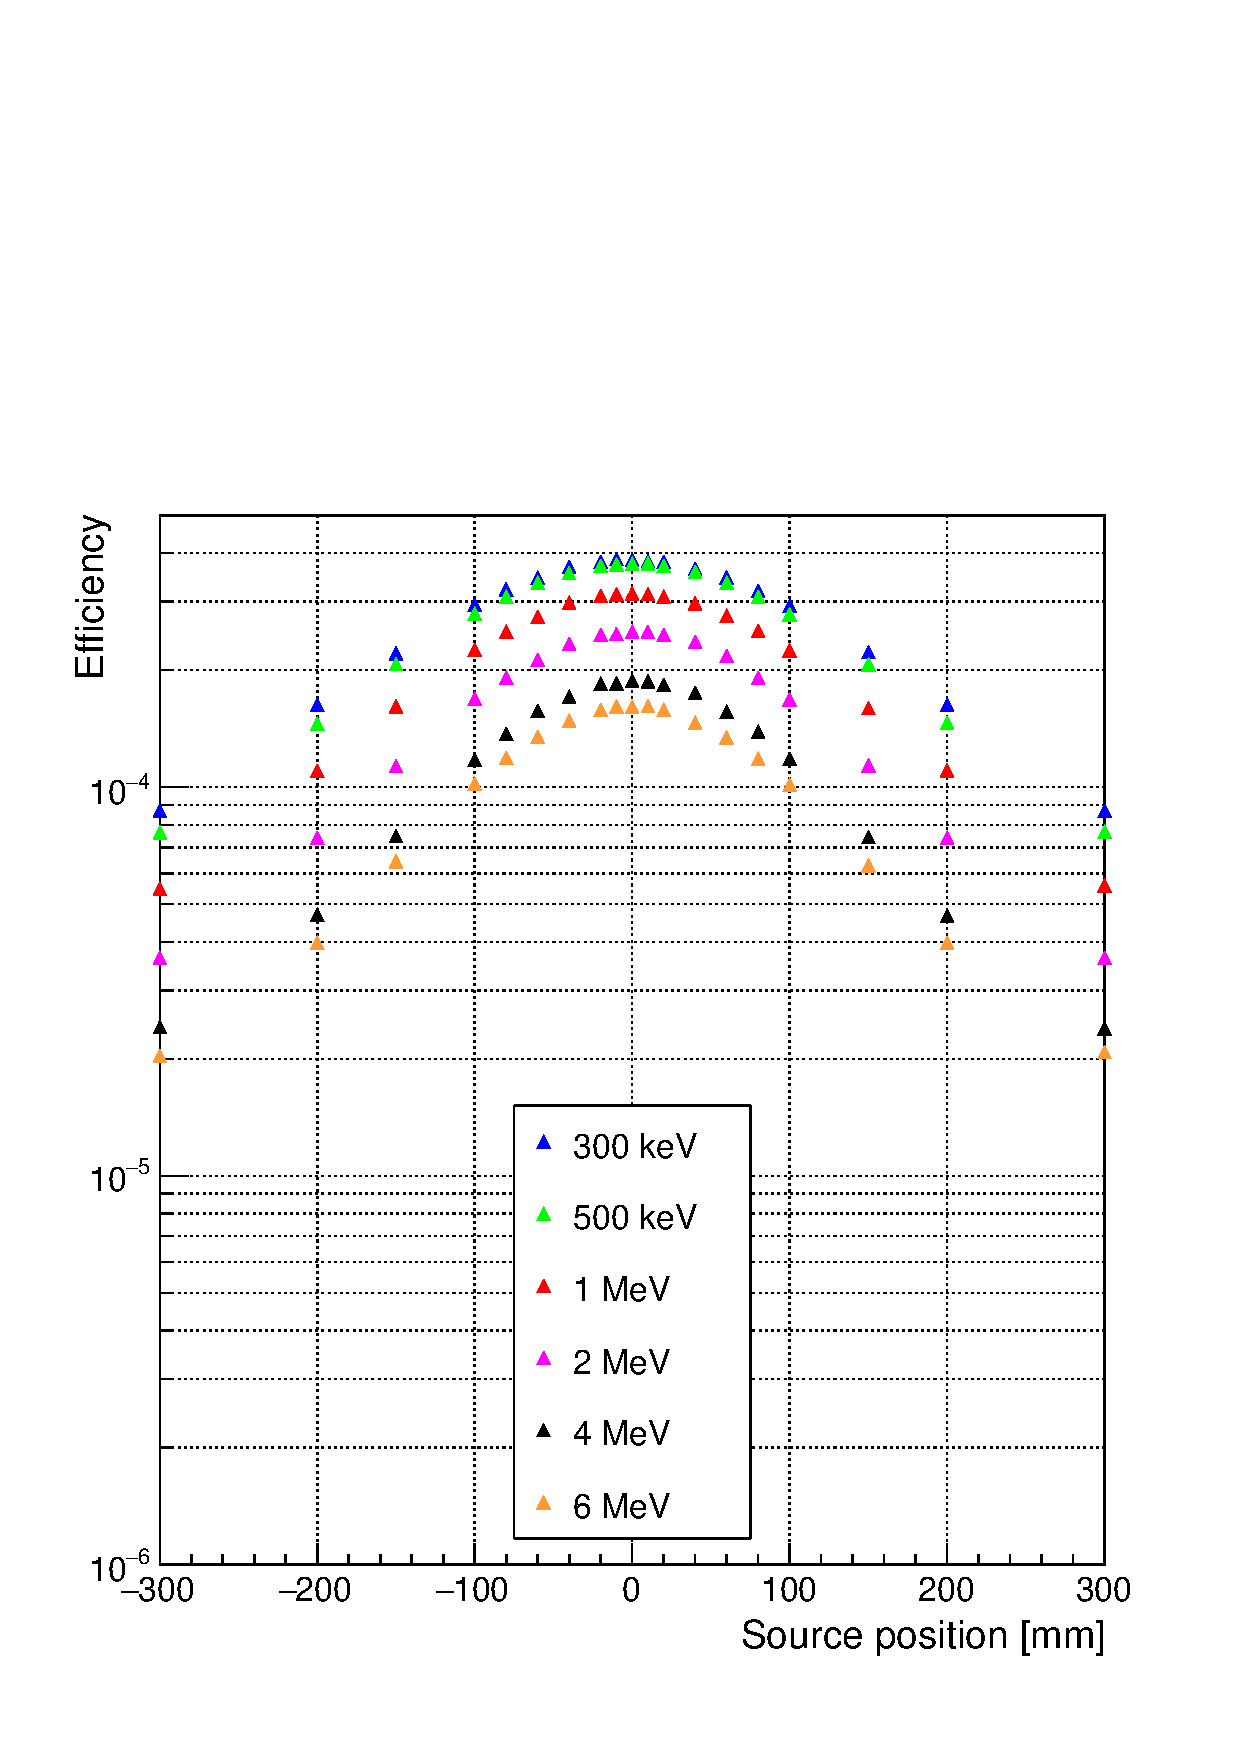
\includegraphics[width=0.5\textwidth]{./Figure/new/EffVSpos_noCut_simple.pdf}}
%\subfloat[]{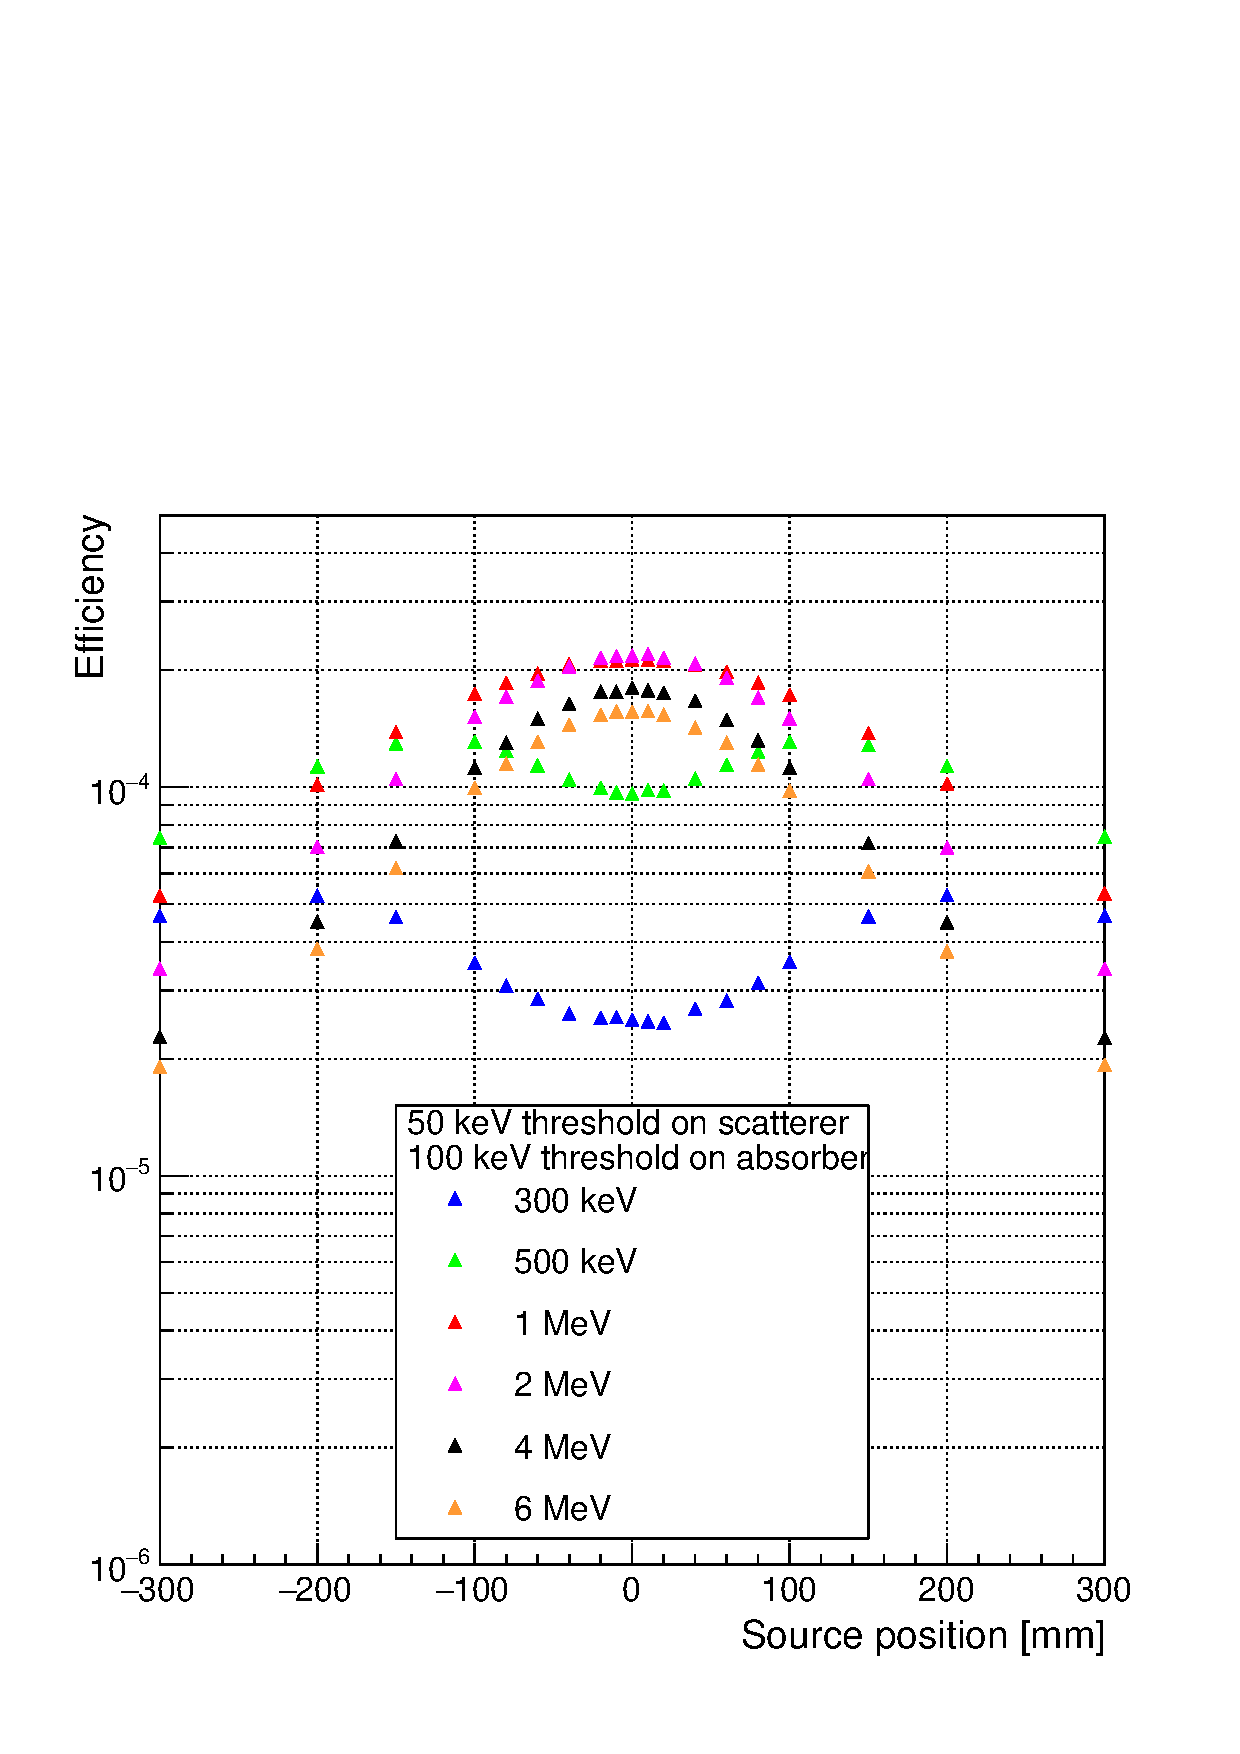
\includegraphics[width=0.5\textwidth]{./Figure/new/EffVSpos_withSingleCut.pdf}}
\subfloat[]{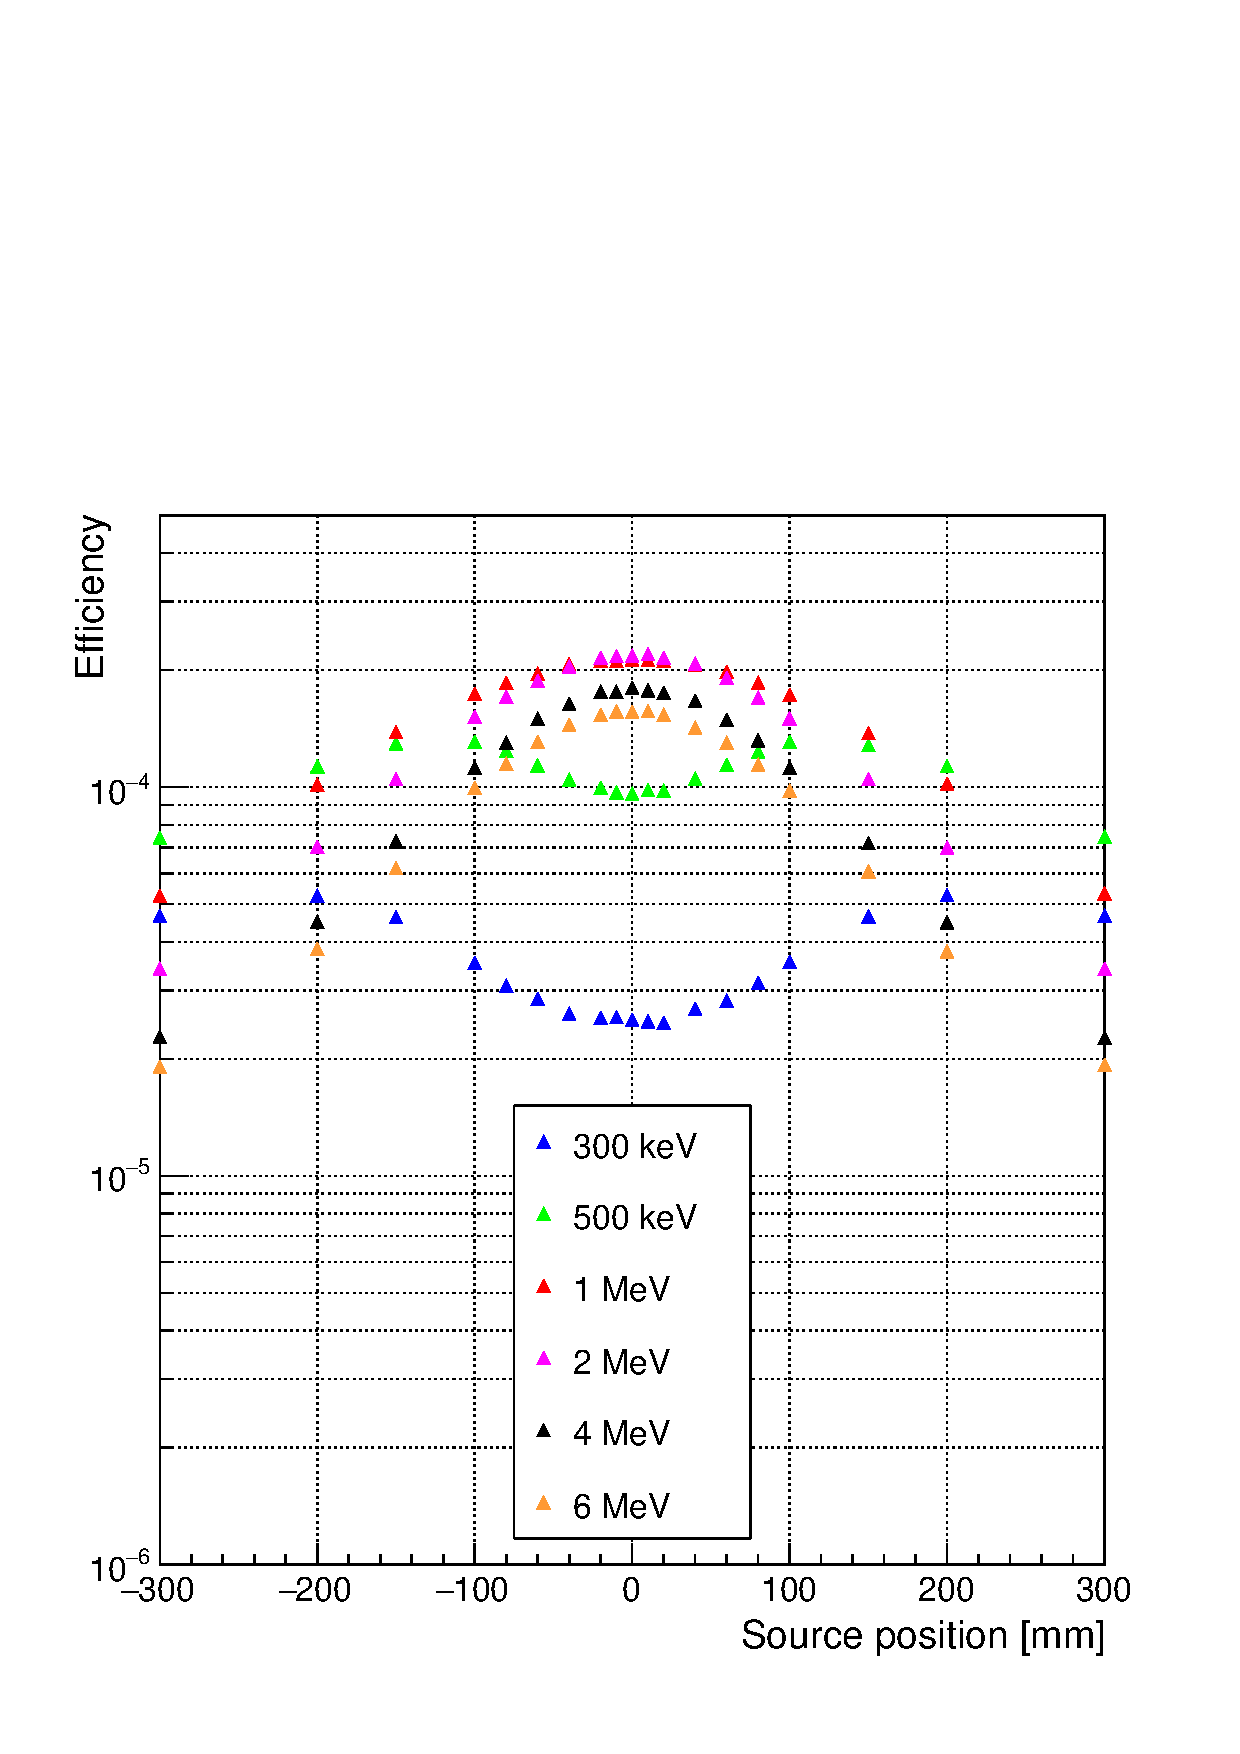
\includegraphics[width=0.5\textwidth]{./Figure/new/EffVSpos_CutSingle_simple.pdf}}
\caption{Absolute Compton camera efficiency as a function of the gamma source position for different gamma energies, in the range between 300~keV to 6~MeV. The left side shows the camera efficiency with no detection energy threshold. In the right side, detection energy thresholds are applied to reproduce a realistic scenario (lower limit of 50~keV for the scatterer, 100~keV for the absorber). These values can change for the final configuration, according to the detector energy resolutions achieved.}
\label{fig::efficiency_study}
\end{figure}

As expected according to the interaction probability energy dependency, the efficiency is higher for low gamma energies, and it lies in the range $4\times10^{-4}$ at 300~keV and $1.5\times10^{-4}$ at 6~MeV at the center of the camera. Moreover, it can be noticed how the efficiency drops as the point source is shifted away from the camera center: efficiency reductions of a factor approximately 4 and 8 at 500~keV and 4~MeV, respectively, are detected with the source at 300~mm distance from the camera center, with respect to the value detected in central position. This effect is more important for high energies, for which the incident gamma is less deflected in the scatterer for the same energy deposited compared to a low energy gamma.   
Figure~\ref{fig::efficiency_study}(b) shows the effect of realistic camera detection thresholds as opposed to the detection without energy thresholds. The gamma detection efficiency drops of a factor ranging from about 1.25 to more than an order of magnitude for the central detection area for energies in the range 300~keV to 2~MeV respectively. The effect is reduced by the distance of the source from the center of the camera. Negligible effects are detected for positions with a distance greater than 200~mm from the center of the camera, and for any distance at energies above 2~MeV, while the efficiency is reduced in the central area of the camera for energies below 4~MeV.\\
 
\subsection{Rate of background coincidences}
\label{Results::beamInt}
 
In Figure~\ref{fig:coincidences}, the different components of the signal resulting from the PMMA exposure to proton and carbon ion beams are shown as a function of the beam intensity. The true coincidences represent scatterer-absorber time coincidences generated by the same gamma ray (only events with hits in a single scatterer layer). All the other coincidence types compose the background. The collected data sets are reported with and without the applied time-of-flight discrimination, mainly employed for neutron rejection, as mentioned in section~\ref{MatMeth::TOF_Ecut}.

\begin{figure} [!h]
  %\subfloat[]{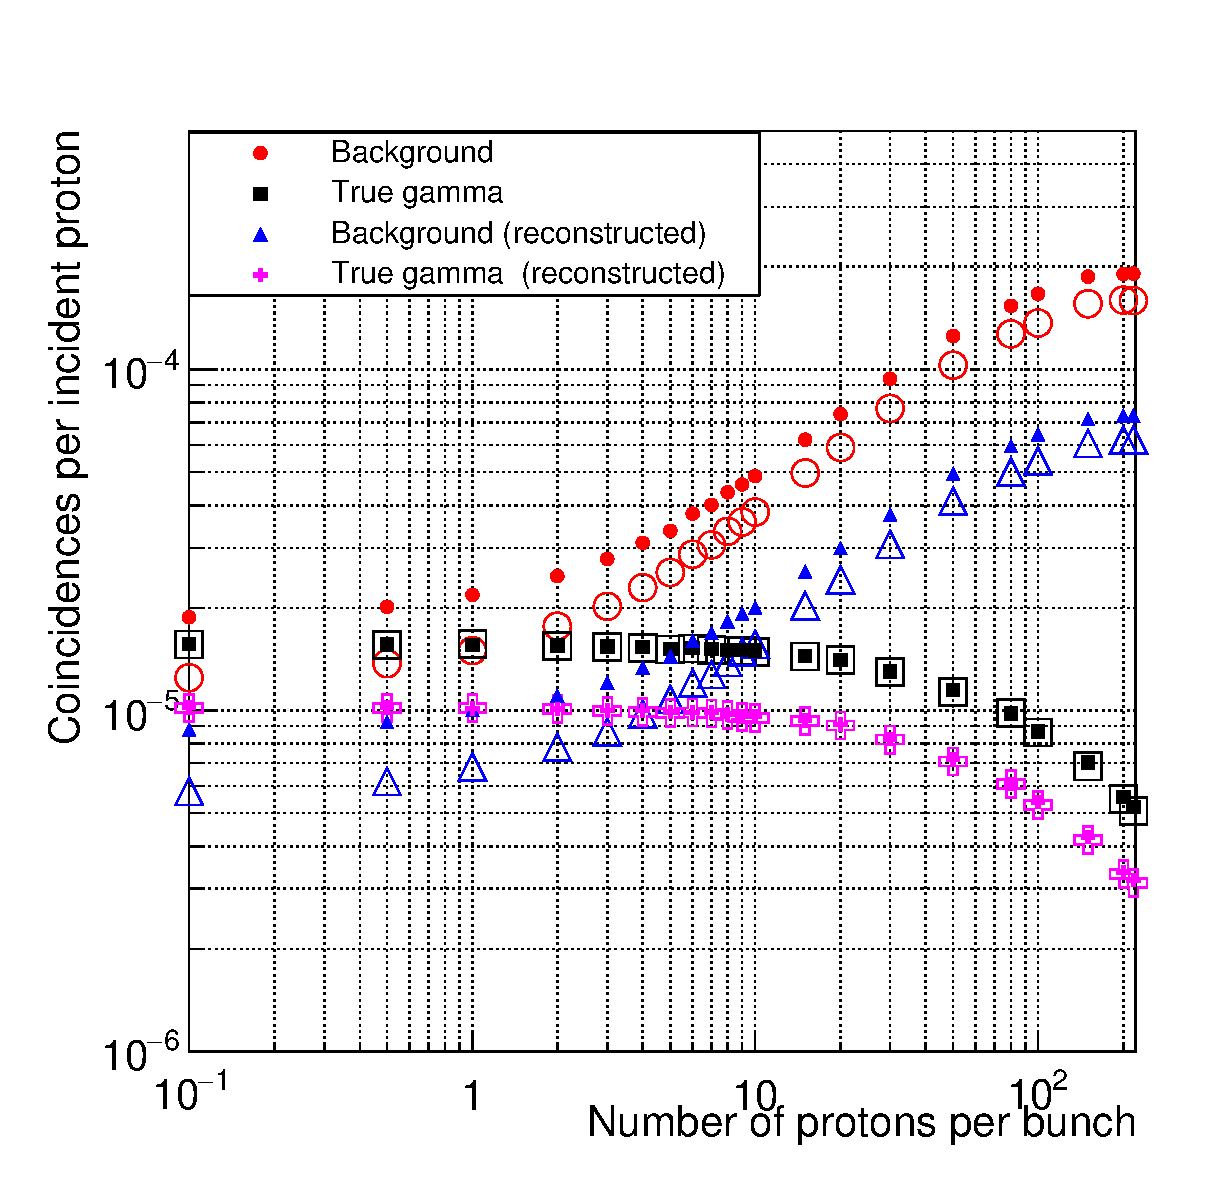
\includegraphics[width=0.5\textwidth]{./Figure/2017_06_28_Taux_coincidences_variation_protons_New_design_4EntreesLegend_LogXLogY.eps}}
  \subfloat[]{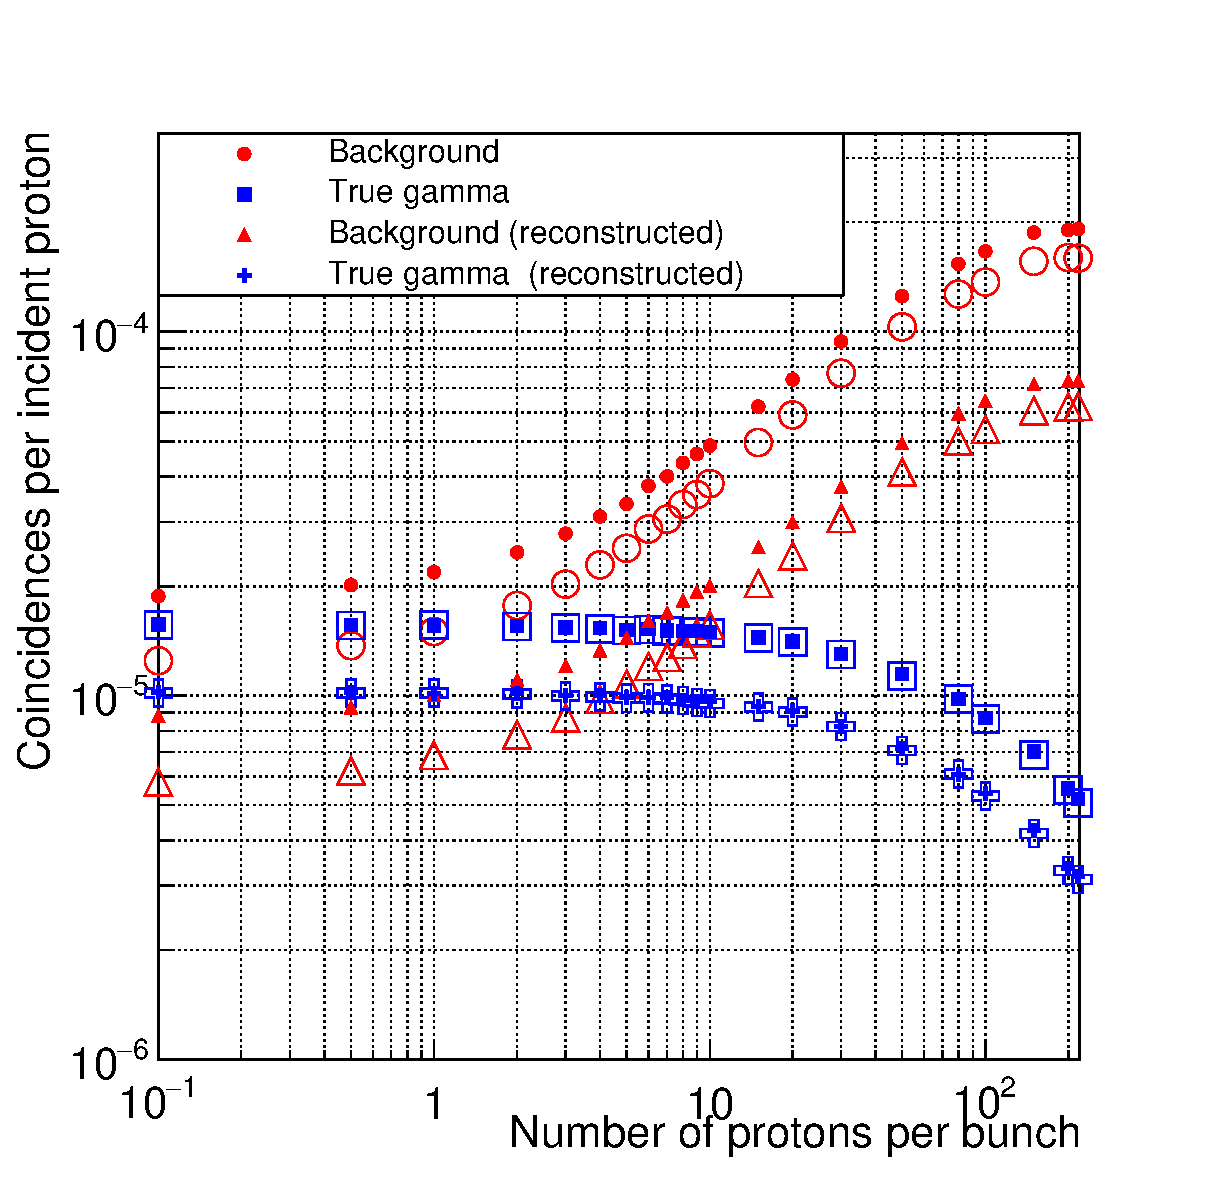
\includegraphics[width=0.5\textwidth]{./Figure/new/coincYields_protons.eps}}
  %\subfloat[]{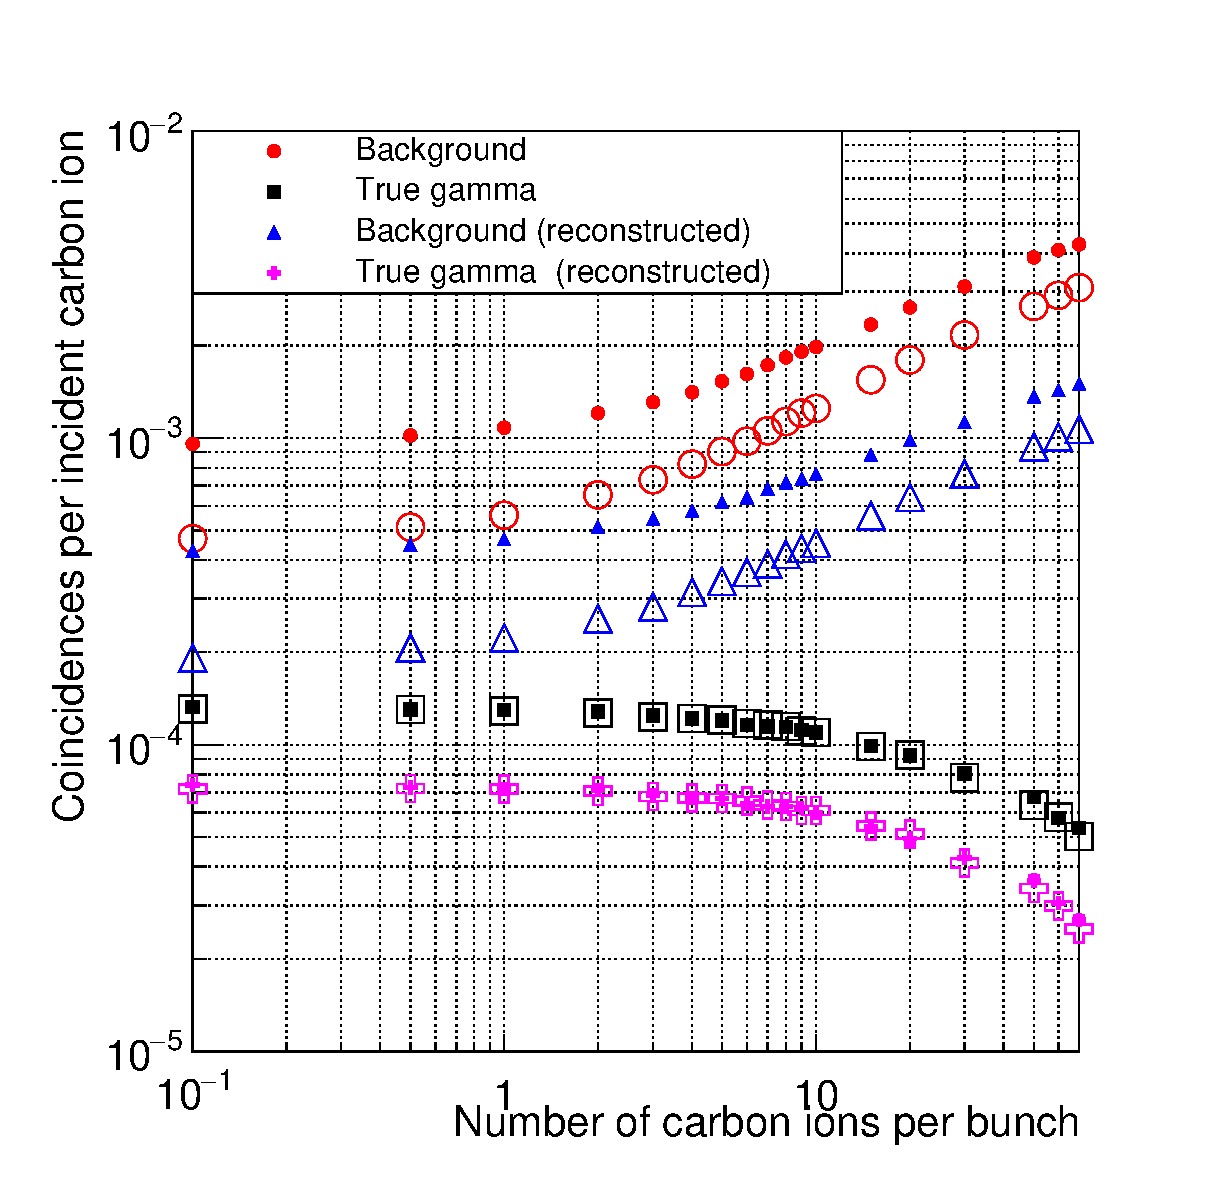
\includegraphics[width=0.5\textwidth]{./Figure/2017_06_28_Taux_coincidences_variation_carbonIons_New_design_4EntreesLegend_LogXLogY.eps}}
  \subfloat[]{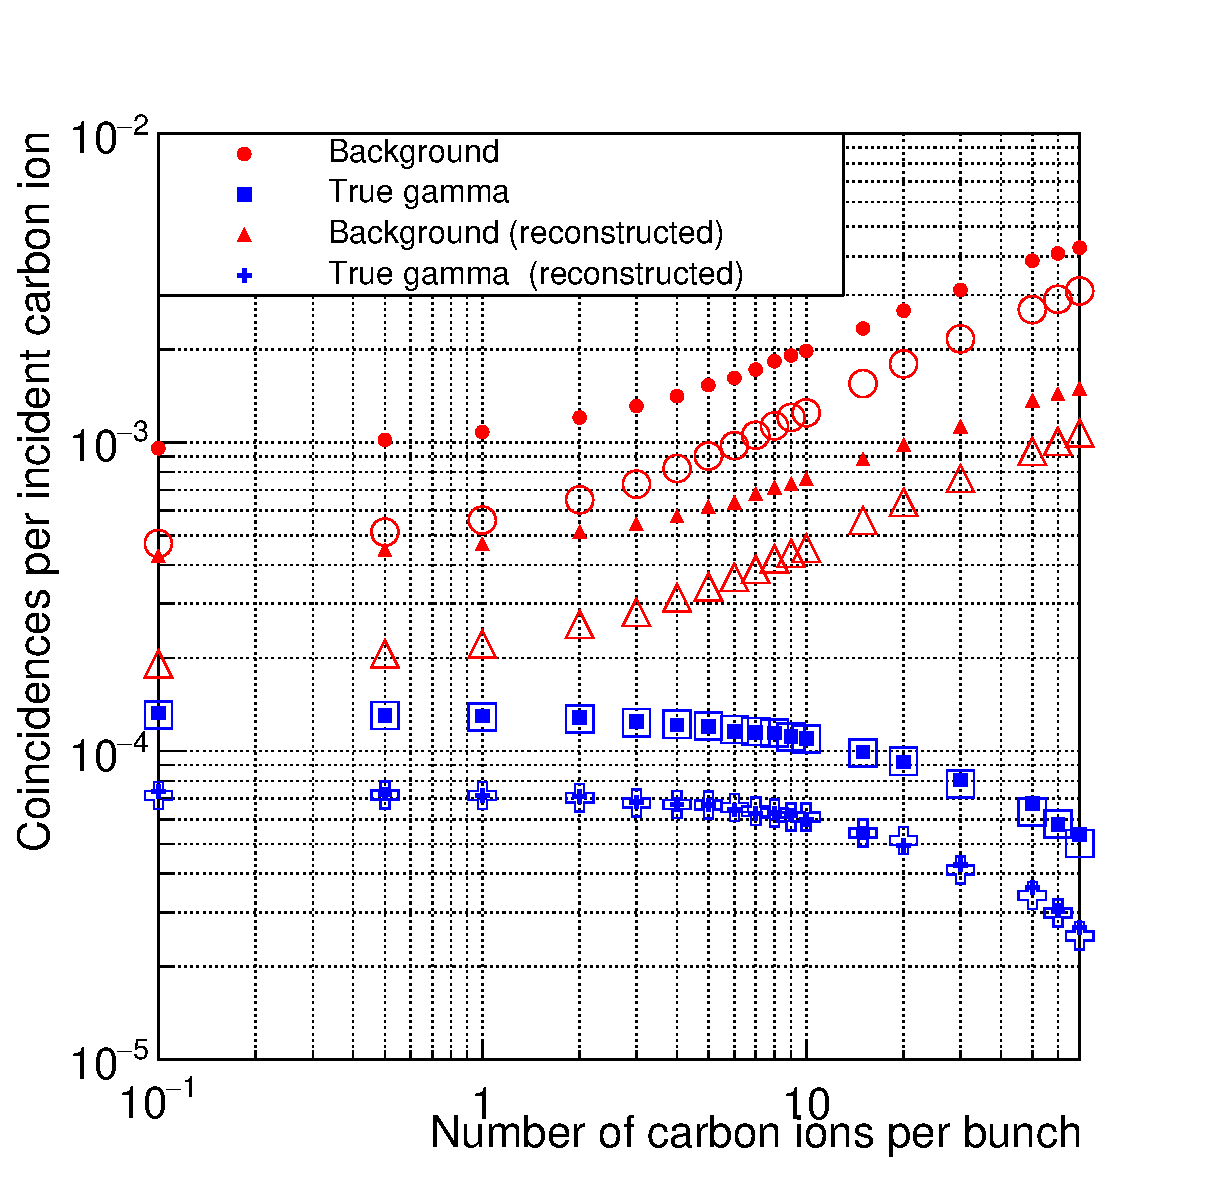
\includegraphics[width=0.5\textwidth]{./Figure/new/coincYields_Cions.eps}}
  \caption{Coincidences yield for protons (left) and carbon ions (right) as a function of the beam intensity. The intensity is reported as number of incident particles per bunch. The filled markers correspond to the collected data without time-of-flight discrimination, while this cut is applied to the data reported with empty markers. Moreover, the yields are given before and after the profile reconstruction with the line-cone algorithm, which rejects events reconstructed out of the target volume.}
  \label{fig:coincidences}
\end{figure}

In Figure~\ref{fig:coincidences}(a) and (b) the amount of true gamma coincidences and background events are reported before and after reconstruction via line-cone algorithm as a function of the beam intensity for proton (a) and carbon ion (b) beams. In addition to this, for each curve realized with the complete collected data set, the related one obtained after time-of-flight selection of events is sketched (empty symbols). All the curves have been normalized to the number of incident ions.

The amount of background events (mainly random coincidences - due to quasi-simultaneous interactions of different gammas) increases with the increasing beam intensity: a factor of about 30 with respect to true gamma events is obtained for proton beams at  the intensity of 200 protons per bunch with no event selection, while a factor more than two times higher is reported for carbon ions in the same conditions. The time-of-flight selection can slightly improve the signal-to-noise ratio by reducing the amount of background events. The amount of true gamma events and background events becomes similar at the intensity of about 1 proton per bunch. As expected by the observation of Figure~\ref{fig:fig_TOF_distribution_CC_simulation_Hadronth}, for intensity values below 1 proton per bunch, the ratio between true and background events remains stable. 


\subsection{Camera precision}
\label{Results::precision_reconstruction}
The camera precision in the fall-off identification is investigated with proton beams.
A data set corresponding to the irradiation of the PMMA phantom with a monoenergetic 160~MeV proton beam spot (10$^8$ protons) has been collected and analyzed with a clinical intensity of 200 protons per bunch and a reduced one with 1 proton per bunch on average. 
Figure~\ref{fig:comparison} shows the results of the line-cone and LM-MLEM reconstructions of the simulated data for the two beam time structures applied at the analysis stage.  

\begin{figure}
\centering
\hspace{-0.7cm}\subfloat[]{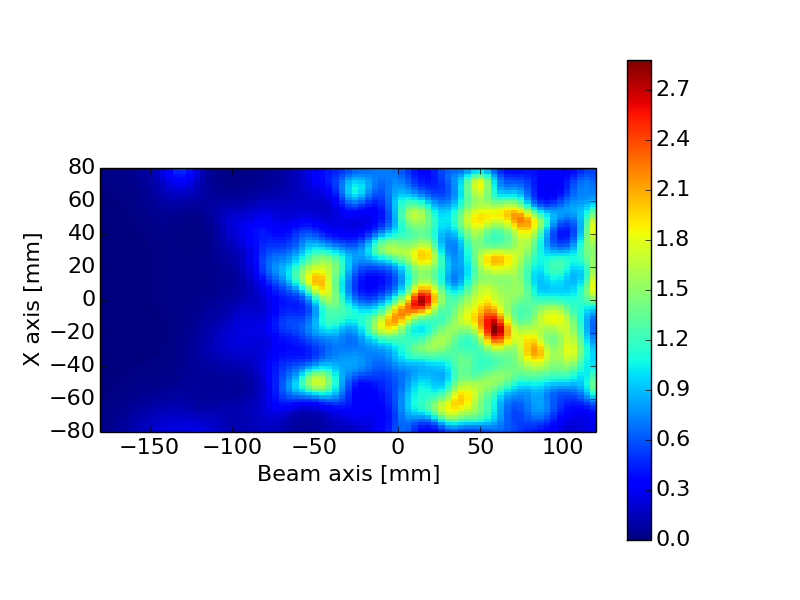
\includegraphics[width=0.41\textwidth,clip=true,trim=0 70 130 90]{./Figure/new/recon_200pBunch/projection2D_Z_corr_r20.png}}
\subfloat[]{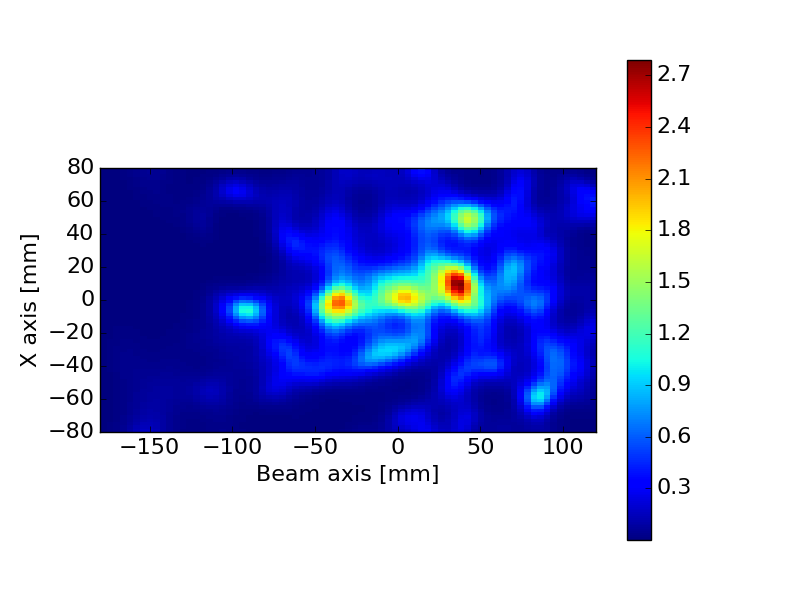
\includegraphics[width=0.41\textwidth,clip=true,trim=0 70 130 90]{./Figure/projection2D_Z_corr_r20.png}}\\
\vspace{-0.45cm}
\subfloat[]{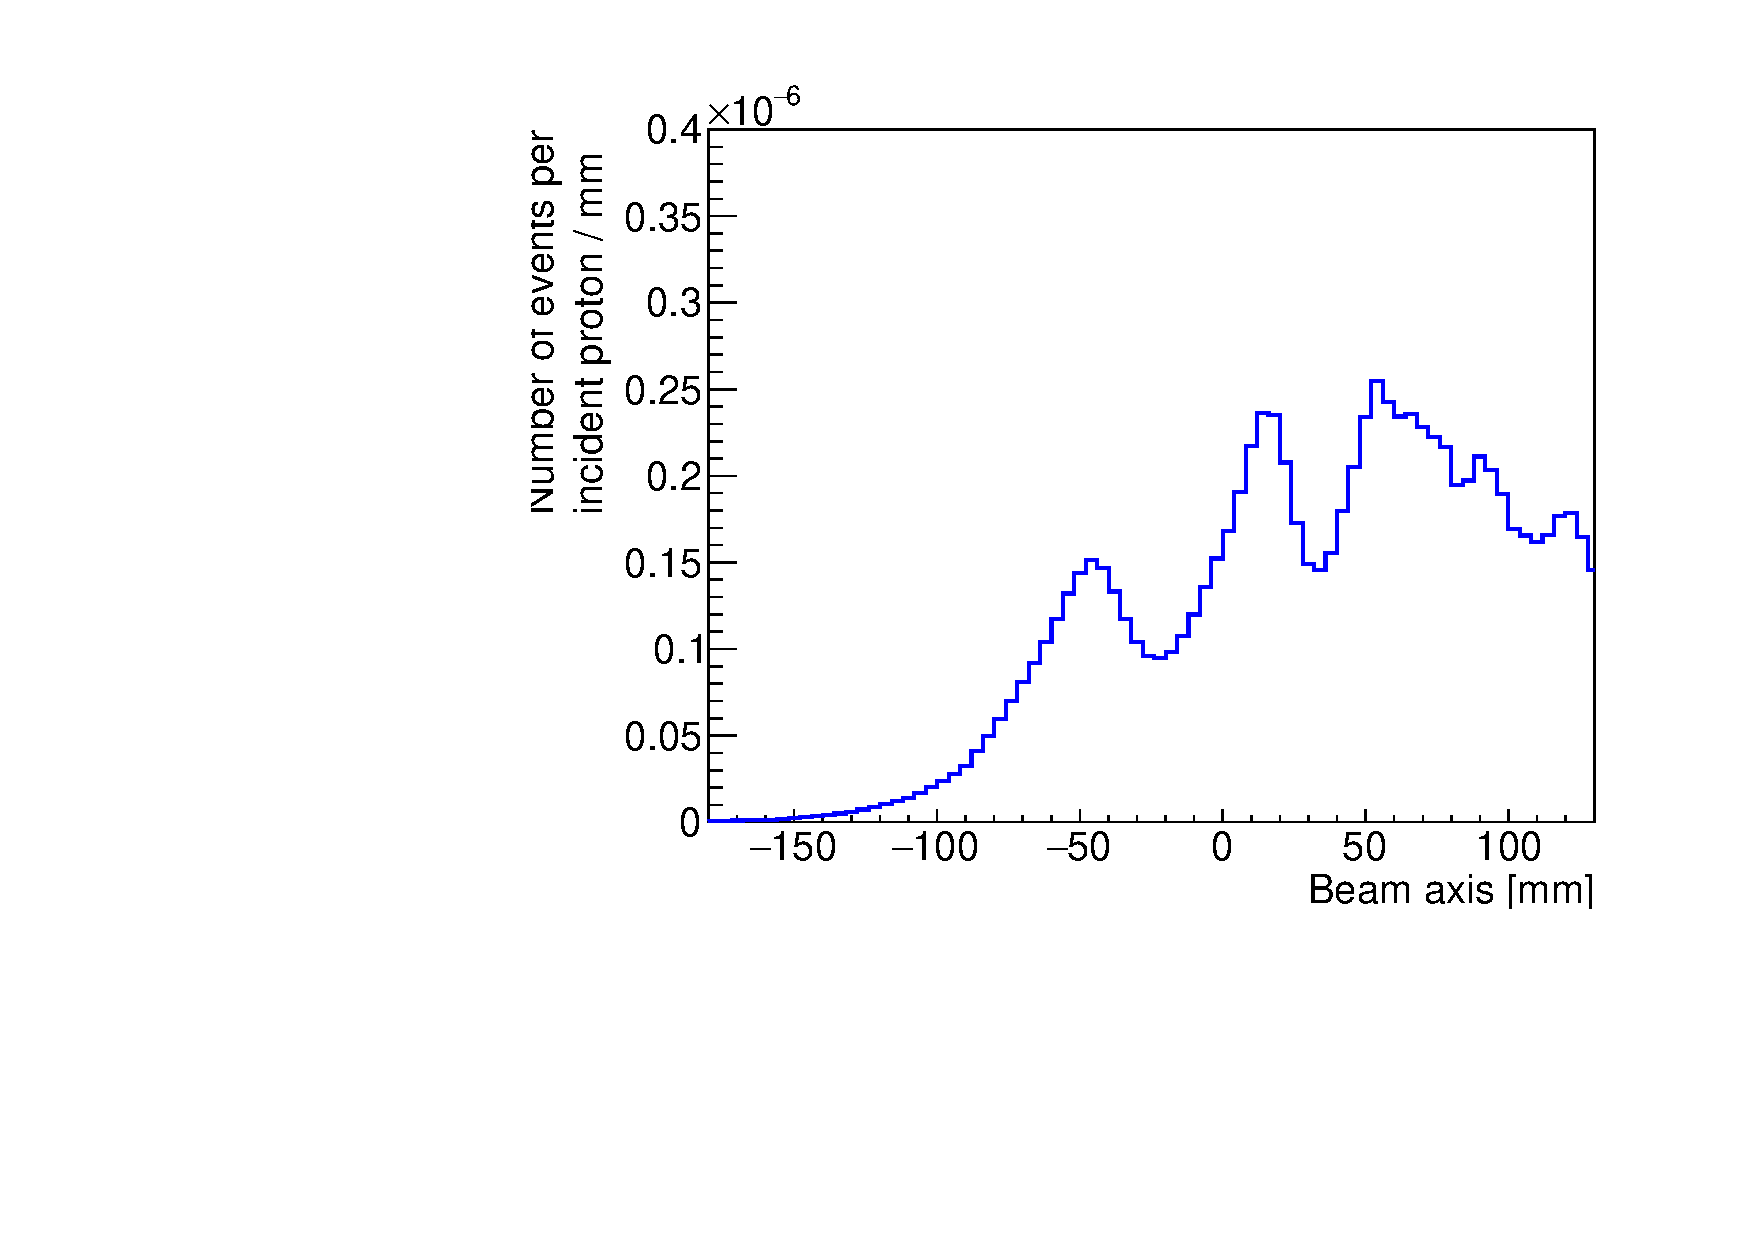
\includegraphics[width=0.41\textwidth]{./Figure/new/profile_MLEM_200pBunch.pdf}}
\subfloat[]{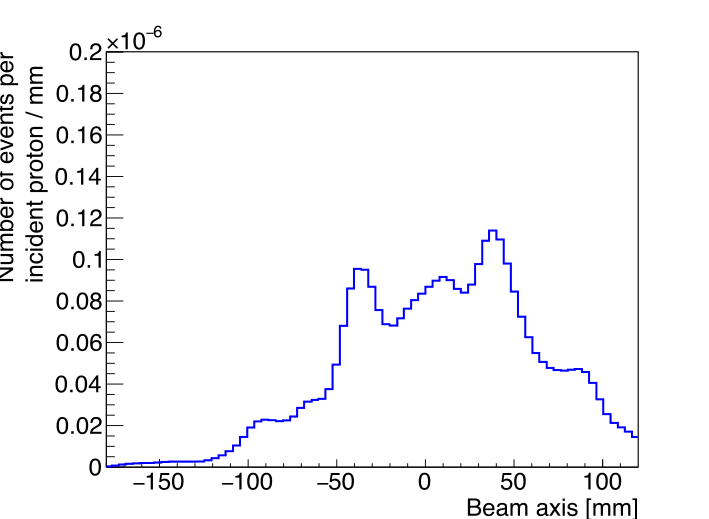
\includegraphics[width=0.41\textwidth]{./Figure/new/reconstructed_lowStat_profile_norm_mod.png}}\\
\vspace{-0.45cm}
\subfloat[]{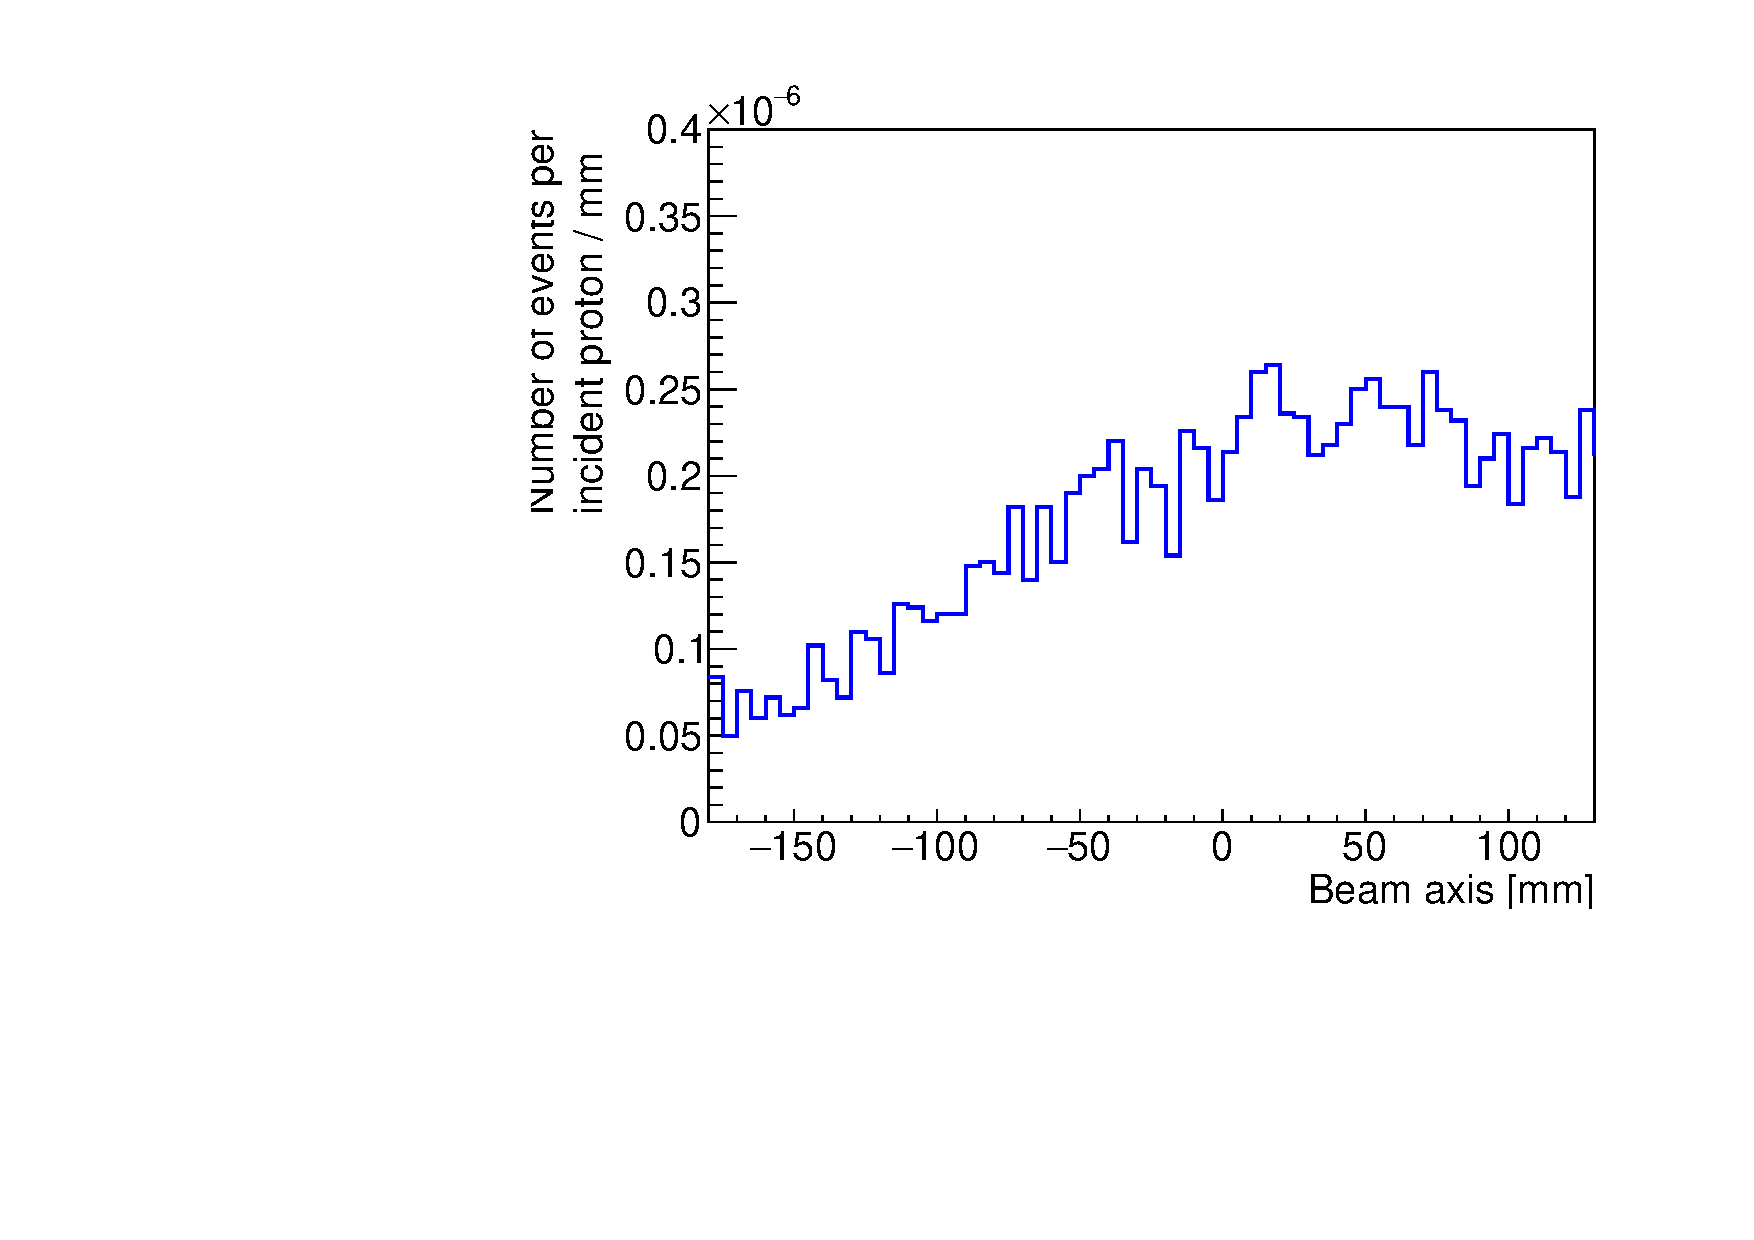
\includegraphics[width=0.41\textwidth]{./Figure/new/profile_lineCone_200pBunch.pdf}}
\subfloat[]{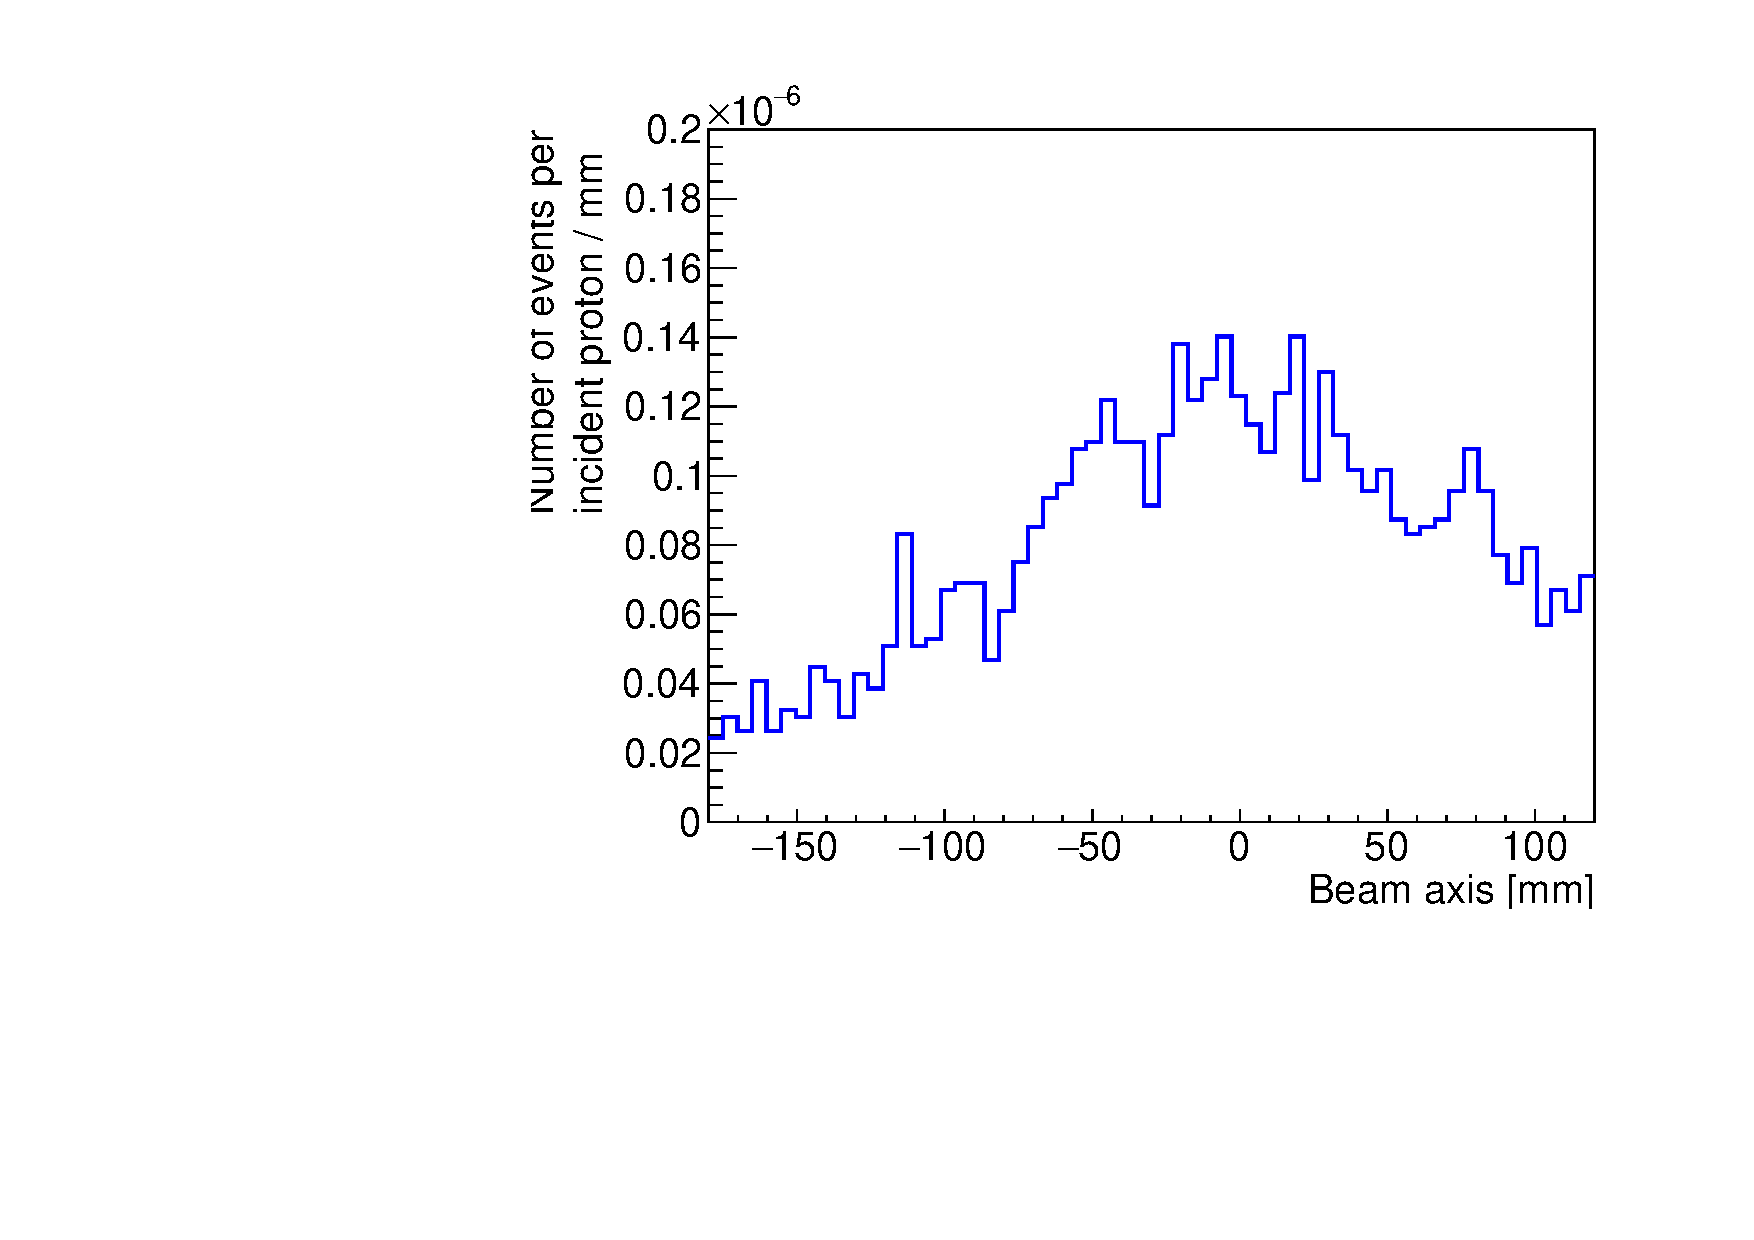
\includegraphics[width=0.41\textwidth]{./Figure/new/recon_profile_line-cone_lowStat_norm.pdf}}
\caption{Line-cone and LM-MLEM reconstruction for a 160~MeV proton beam, $10^{8}$ total incident protons. In the left column, the beam intensity is 200 proton per bunch on average; in the right one, the beam intensity is 1 proton per bunch on average. The Compton camera is centered at the expected Bragg peak position, $y=+50\,$mm. The time-of-flight event selection is applied on the collected data set. 2 iterations are performed for the LM-MLEM reconstruction. The top row shows the MLEM reconstructed 2D images in the plane $(x,y)$, parallel to the camera entrance surface. The position $x=0\,$mm corresponds to the center of the PMMA phantom and the $y$ direction corresponds to the beam axis, with the target entrance at $y=-100\,$mm and the target end at $y=+100\,$mm.  The center row shows the 1D profiles along the $y$ axis. The expected profile fall-off is located at $y=+50\,$mm. The bottom row shows the profiles obtained by means of the line-cone algorithm for the same time-of-flight selected data.}
\label{fig:comparison}
\end{figure}

The results obtained for a clinical intensity of 200 protons per bunch qualitatively show how the fall-off of the prompt-gamma profile cannot be retrieved with the two applied reconstruction methods, due to the contamination of background events. The fall-off can be identified at the reduced intensity of 1 proton per bunch for both line-cone and LM-MLEM reconstructed data.
For this reason, the camera precision is studied at the reduced intensity of 1 proton per bunch on average, at which a comparable rate of true and background events is expected, following the results shown in section~\ref{Results::beamInt}.

Figure~\ref{fig::profilesOverlap} shows the PG profiles obtained for four incident proton statistics in the explored range (10$^{8}$, 5$\times$10$^{8}$, 10$^{9}$, 5$\times$10$^{9}$), reconstructed with the LM-MLEM iterative algorithm, for different numbers of iterations, in the range [1,20].

\begin{figure}
\centering
\subfloat[\label{fig::profilesOver10_8}]{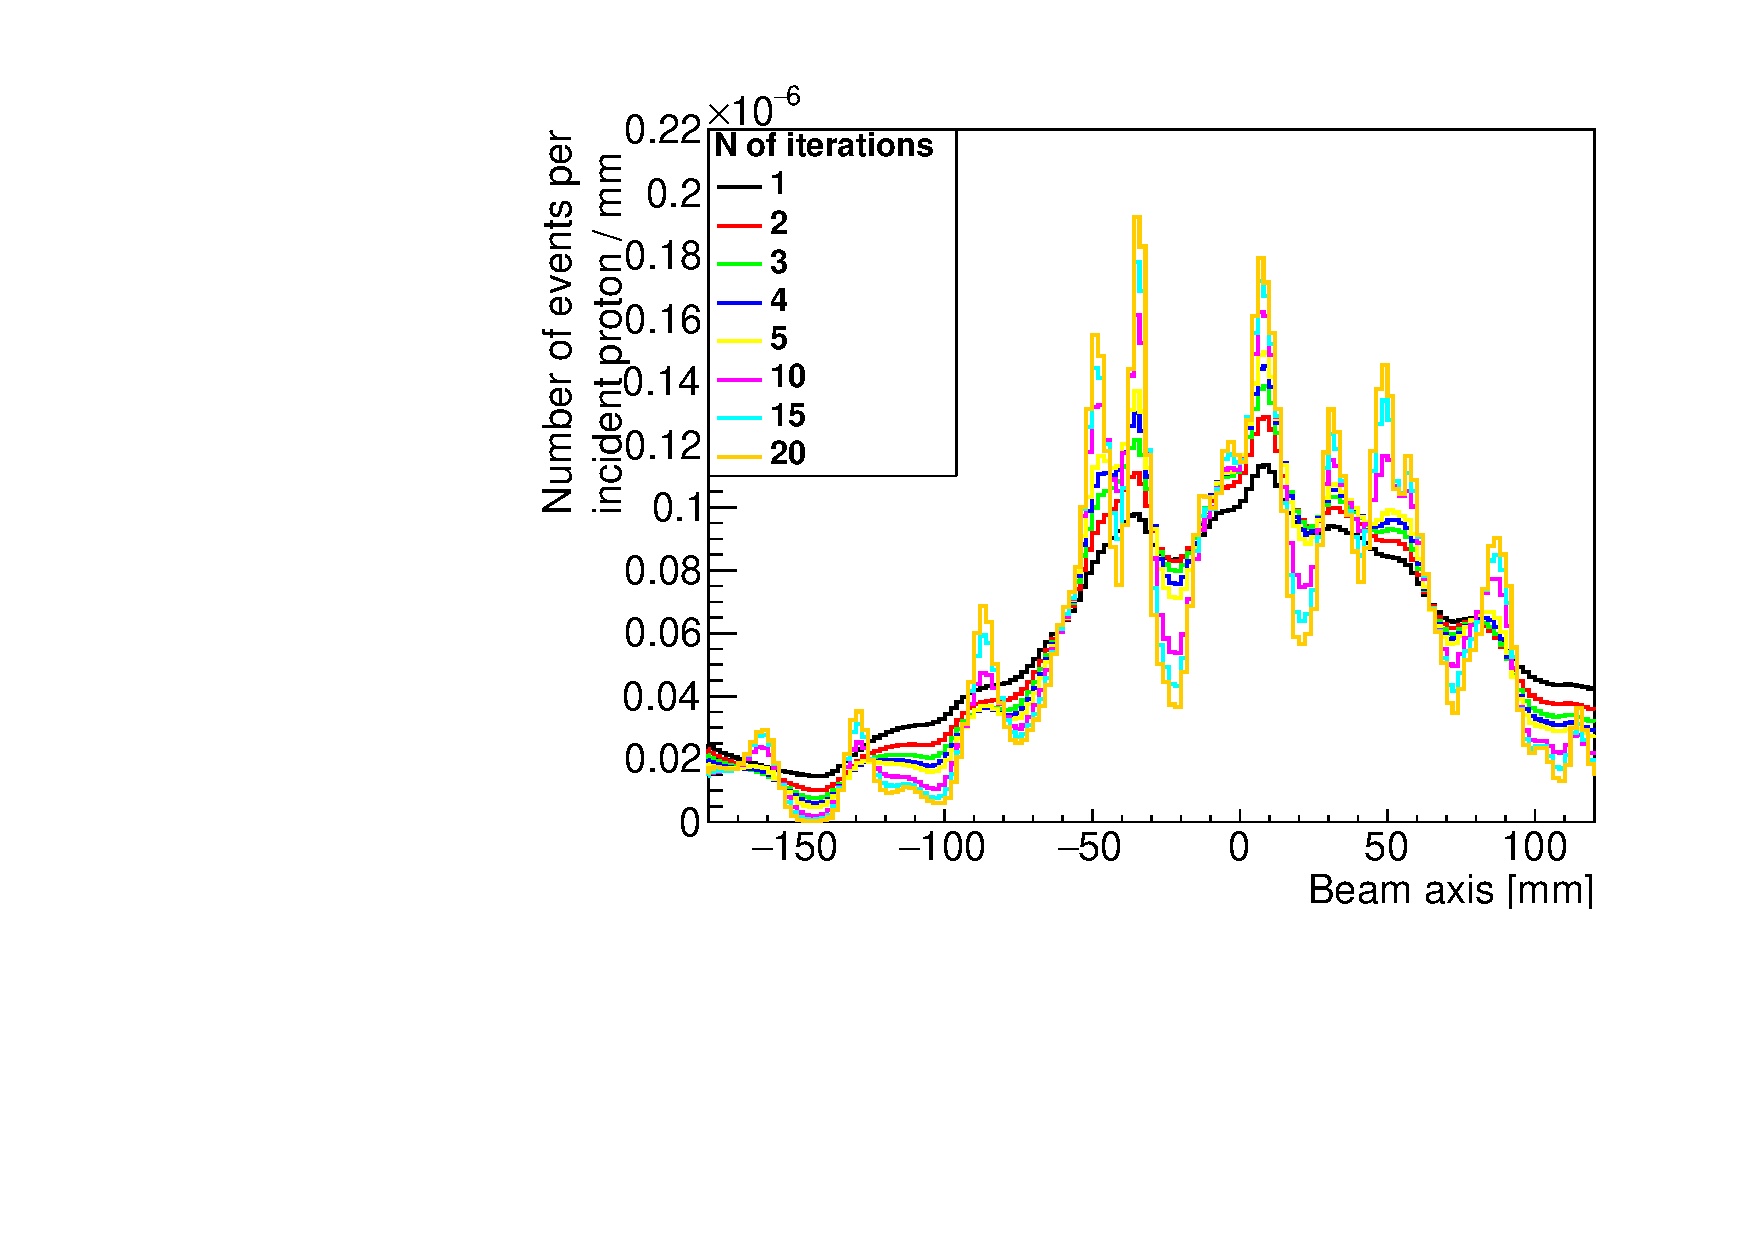
\includegraphics[width=0.45\textwidth]{./Figure/profilesOverlap_10_8_protons.pdf}} 
\subfloat[\label{fig::profilesOver5_10_8}]{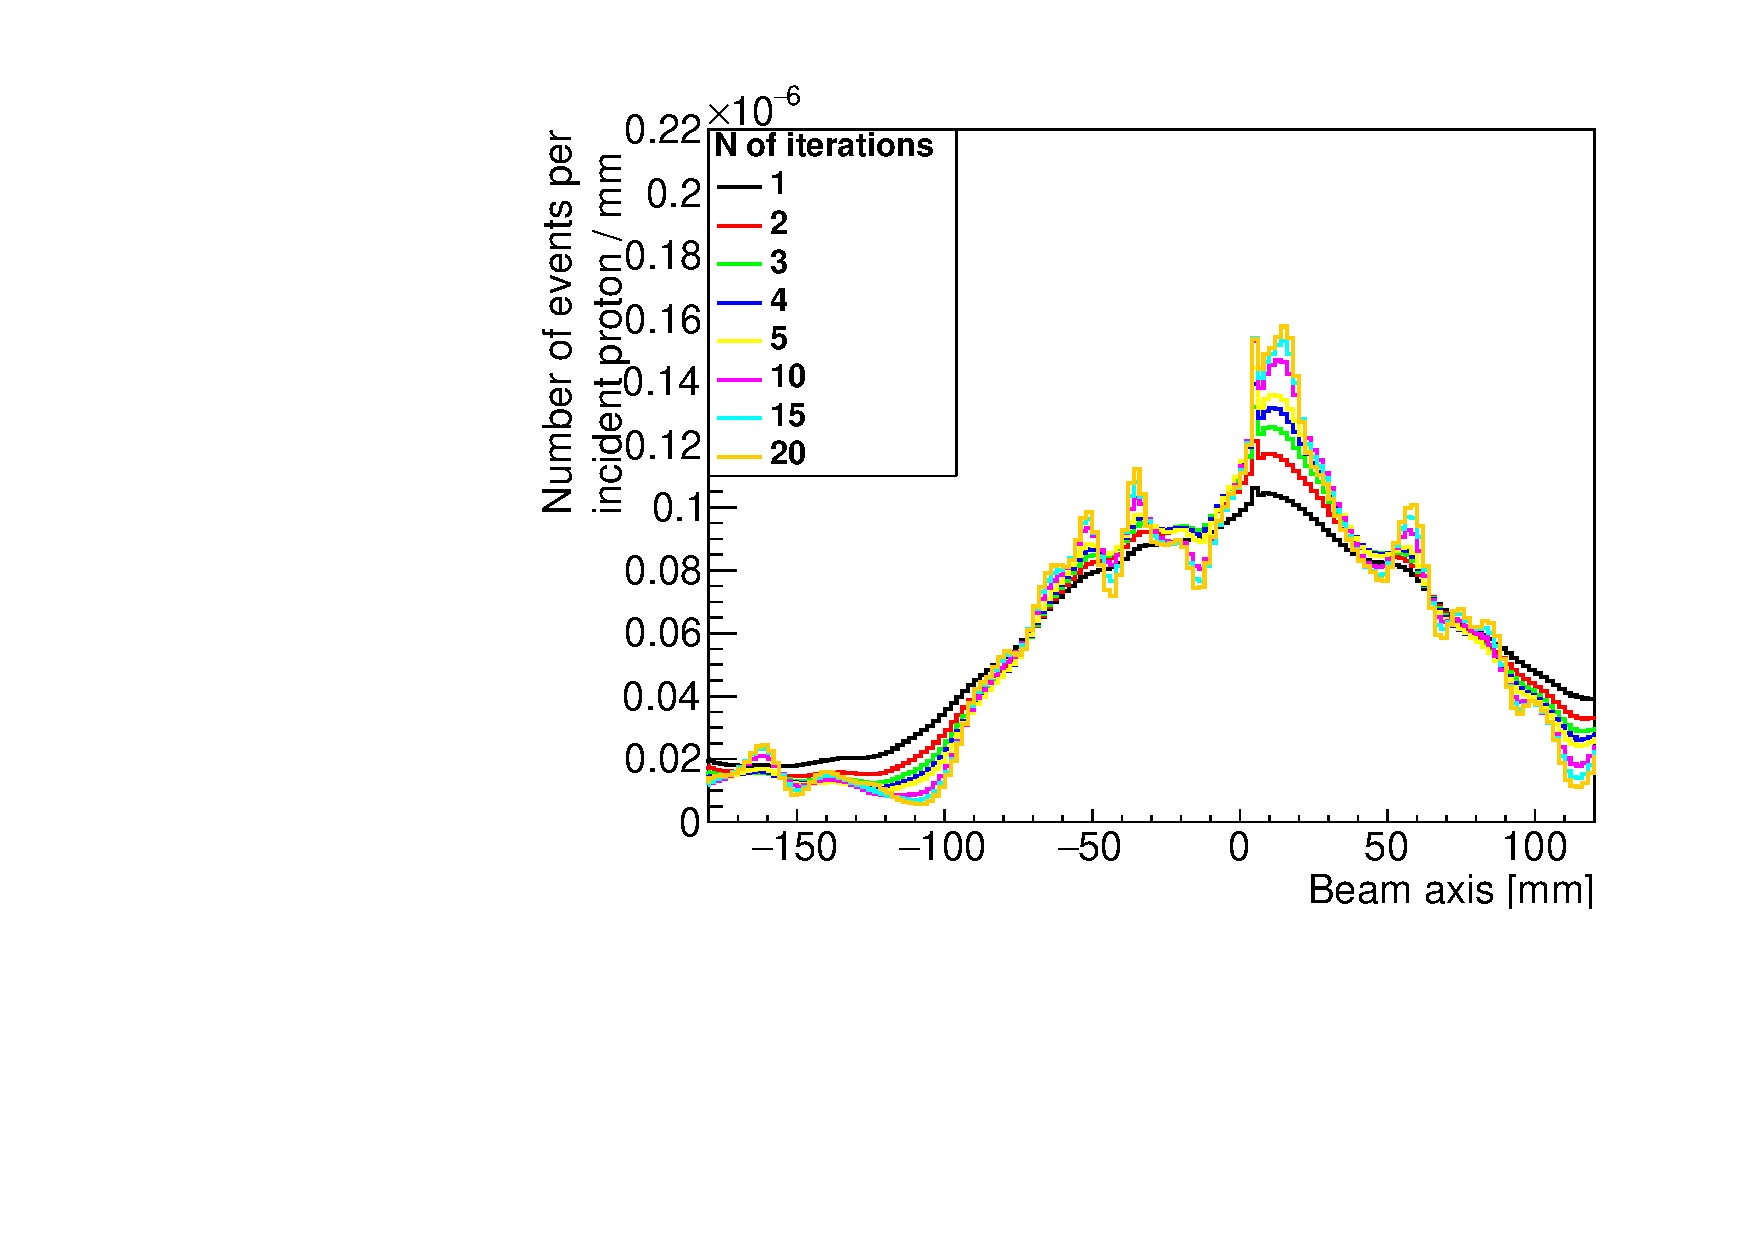
\includegraphics[width=0.45\textwidth]{./Figure/profilesOverlap_5_10_8_protons.pdf}}\\
\subfloat[\label{fig::profilesOver10_9}]{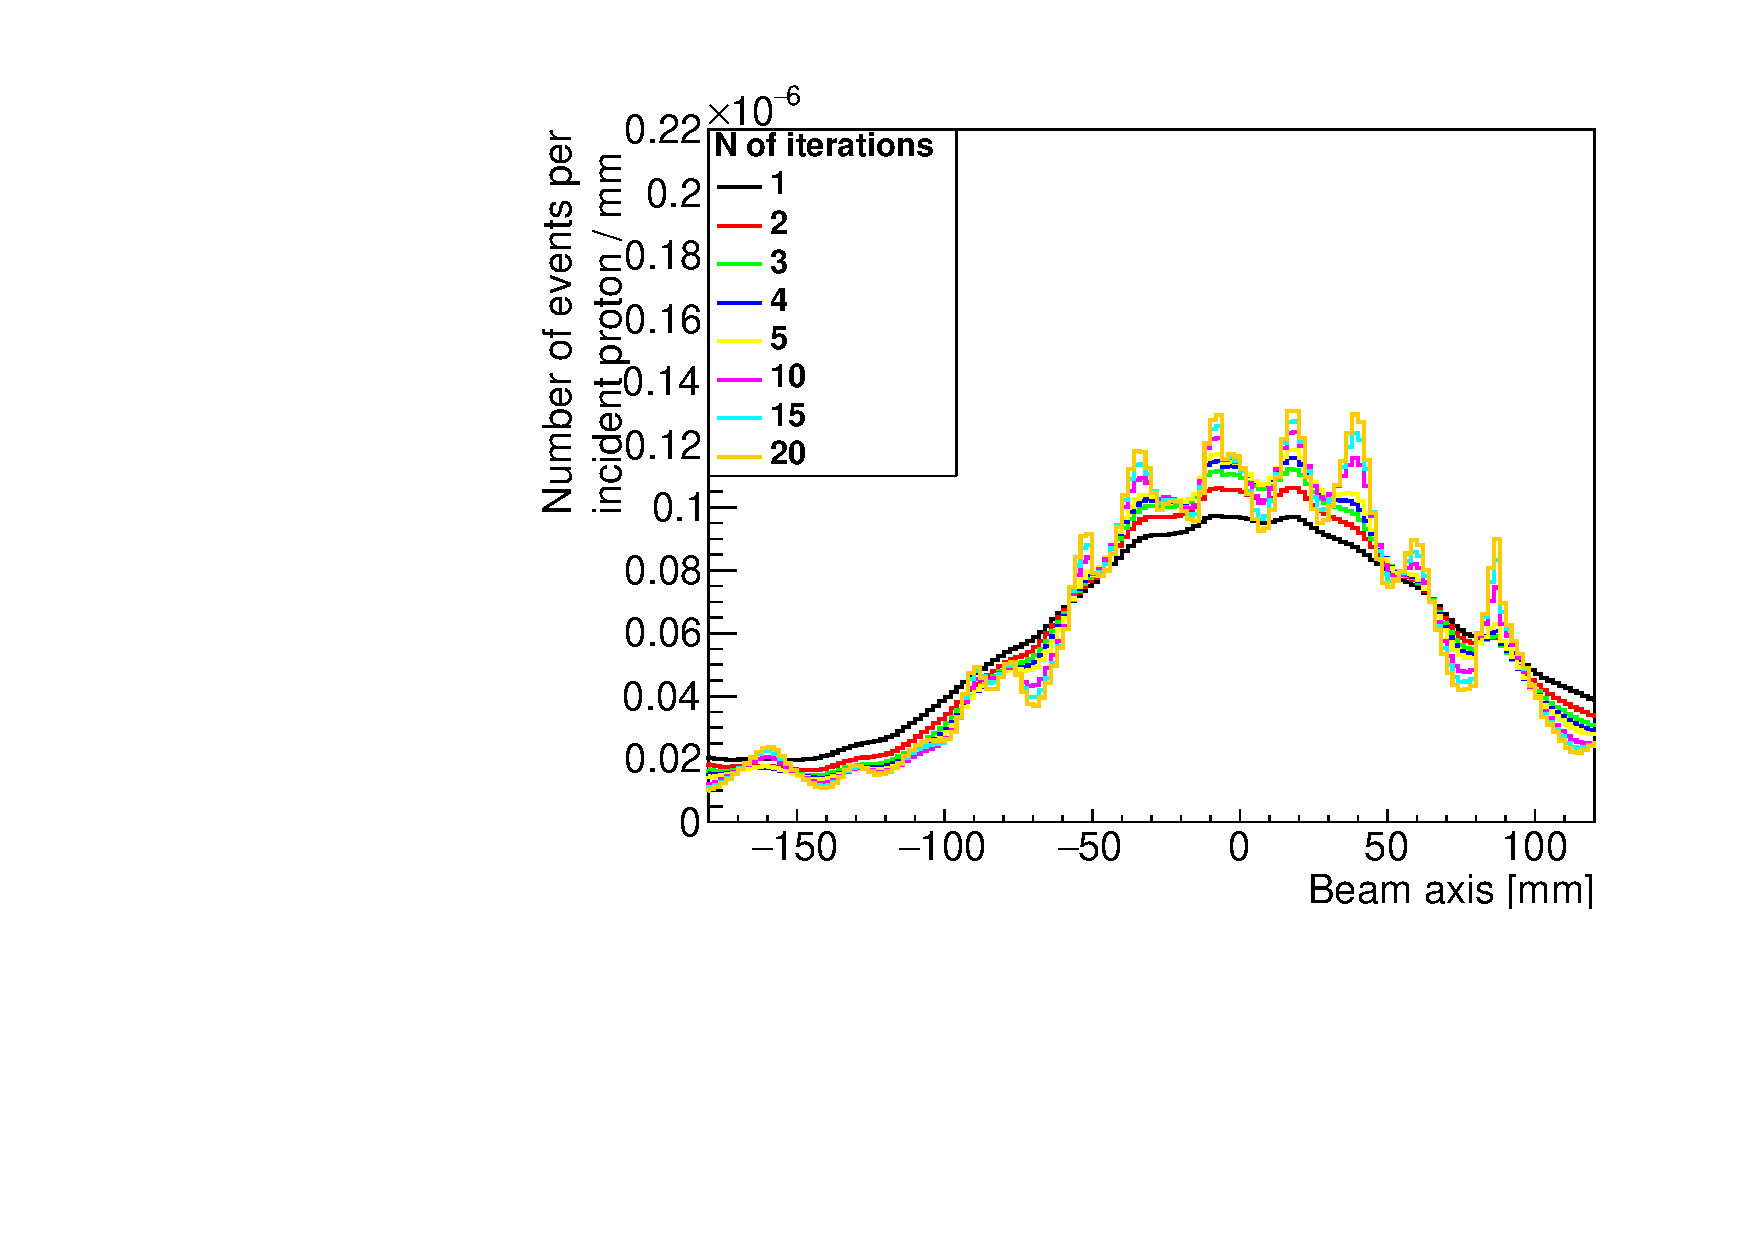
\includegraphics[width=0.45\textwidth]{./Figure/profilesOverlap_10_9_protons.pdf}}
\subfloat[\label{fig::profilesOver5_10_9}]{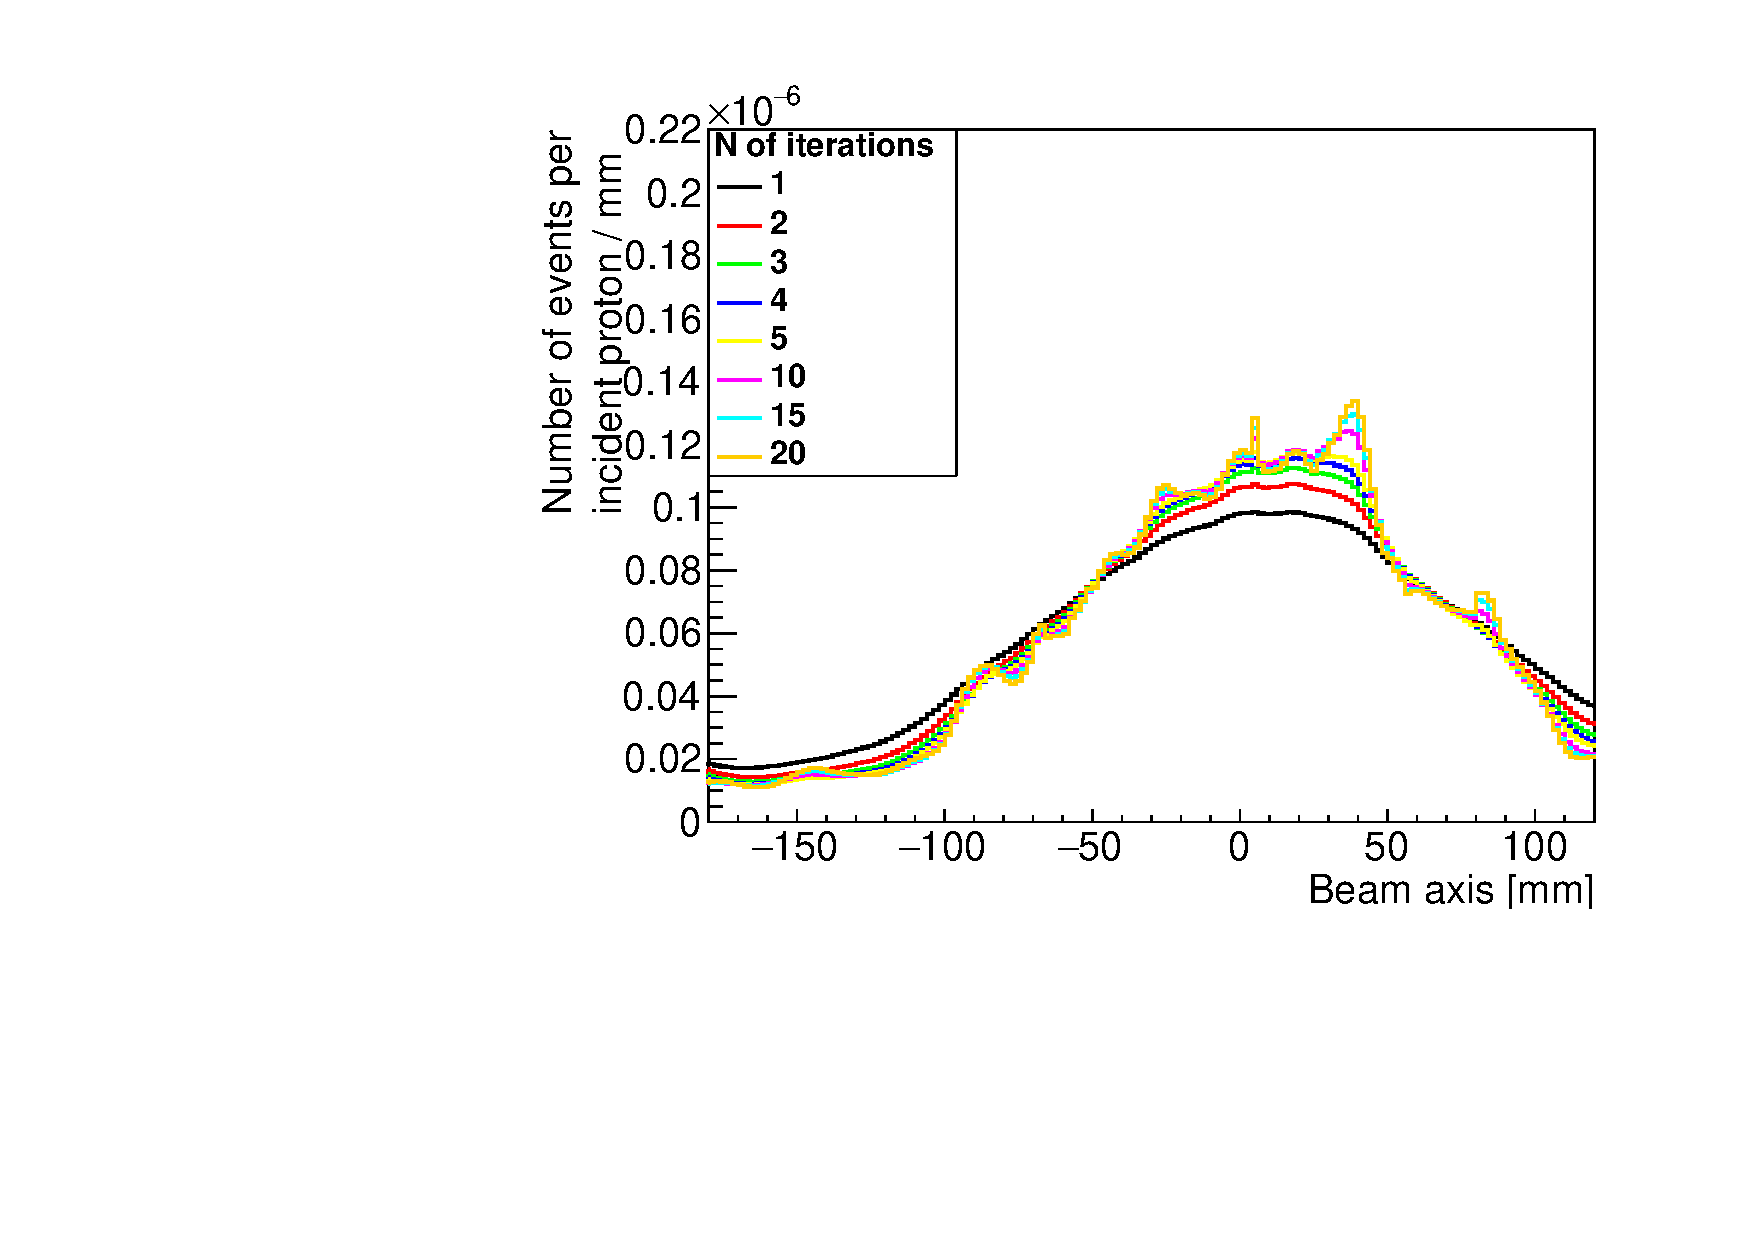
\includegraphics[width=0.45\textwidth]{./Figure/profilesOverlap_5_10_9_protons.pdf}}
\caption{PG profiles for 10$^{8}$ (a), 5$\times$10$^{8}$ (b), 10$^{9}$ (c), and 5$\times$10$^{9}$ (d) incident protons reconstructed with the LM-MLEM algorithm, for 1, 2, 3, 4, 5, 10, 15, 20 iterations.}
\label{fig::profilesOverlap}
\end{figure}

The presented profiles show the effect of the increasing number of iterations of the reconstruction algorithm, which tends to concentrate the emission vertexes in \enquote{hot-spots} creating artifacts which bias the identification of the profile fall-off, mainly at the lowest explored primary statistics. The profile fall-off can be identified with minimized artifacts after 2 iterations of the LM-MLEM algorithm. For this reason, 2 iterations are used for the precision study.

A total of 2$\times10^{10}$ protons has been simulated to define the reference PG profile, with a beam intensity of 1 proton per bunch on average, and then different low statistics profiles have been produced for the precision estimate as explained in section~\ref{MatMeth:precision} for both the line-cone and the LM-MLEM reconstructions. 
The high statistics profile reconstructed via line-cone algorithm is shown in Figure~\ref{fig:fig_Results_Estimation_Camera_Profil_highStat_CC_simulation_Hadronth_LineCone} and via the LM-MLEM reconstruction method in Figure~\ref{fig:fig_Results_Estimation_Camera_Profil_highStat_CC_simulation_Hadronth_MLEM} with the related NURBS fit. A NURBS fit of a low statistics sample ($10^8$ incident protons) is shown in Figures~\ref{fig:fig_Estimation_Camera_CC_NURBS_Poisson_LC} for the line-cone and~\ref{fig:fig_Estimation_Camera_CC_NURBS_Poisson_MLEM} for the LM-MLEM. Poisson extracted fluctuations have been added to the fit curve in the range 30-70~mm (where the fall-off position is expected to be located) for the line-cone case, while the low statistic profile for the LM-MLEM case is obtained with the extraction of a data subset from the reference profile data set and shown together with the reference profile related NURBS.
The retrieved optimal shift distribution is shown in Figure~\ref{fig:fig_Results_Precision_Distribution_Variation_CC_simulation_Hadronth_LC} and~\ref{fig:fig_Results_Precision_Distribution_Variation_CC_simulation_Hadronth_MLEM} for the line-cone and LM-MLEM algorithm respectively, for $10^8$ incident protons as well.

\begin{figure}
\centering
%\subfloat[\label{fig:fig_Results_Estimation_Camera_Profil_highStat_CC_simulation_Hadronth_LineCone}]{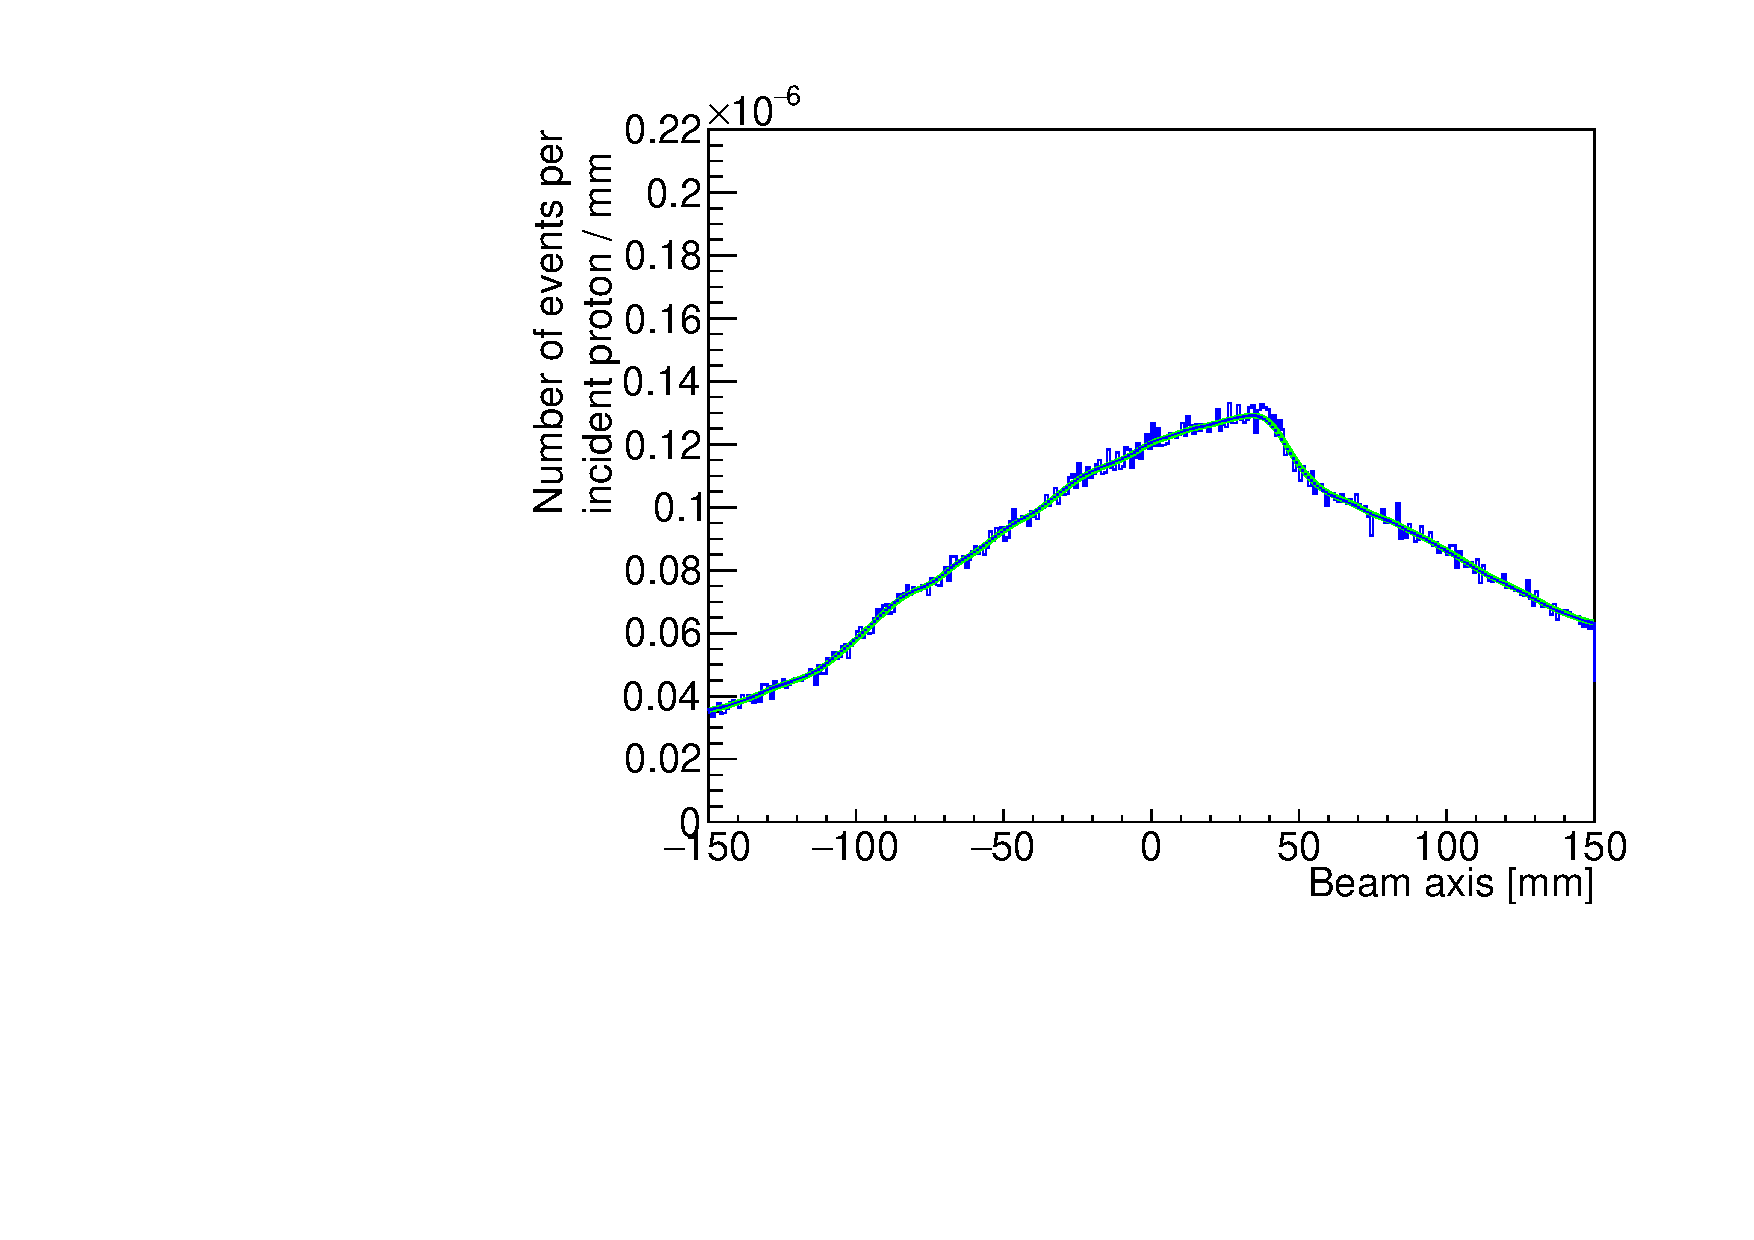
\includegraphics[width=0.48\textwidth]{./Figure/Results_forHadronthPaper/RefProfile_lineCone_plusNurbs.pdf}} 
\subfloat[\label{fig:fig_Results_Estimation_Camera_Profil_highStat_CC_simulation_Hadronth_LineCone}]{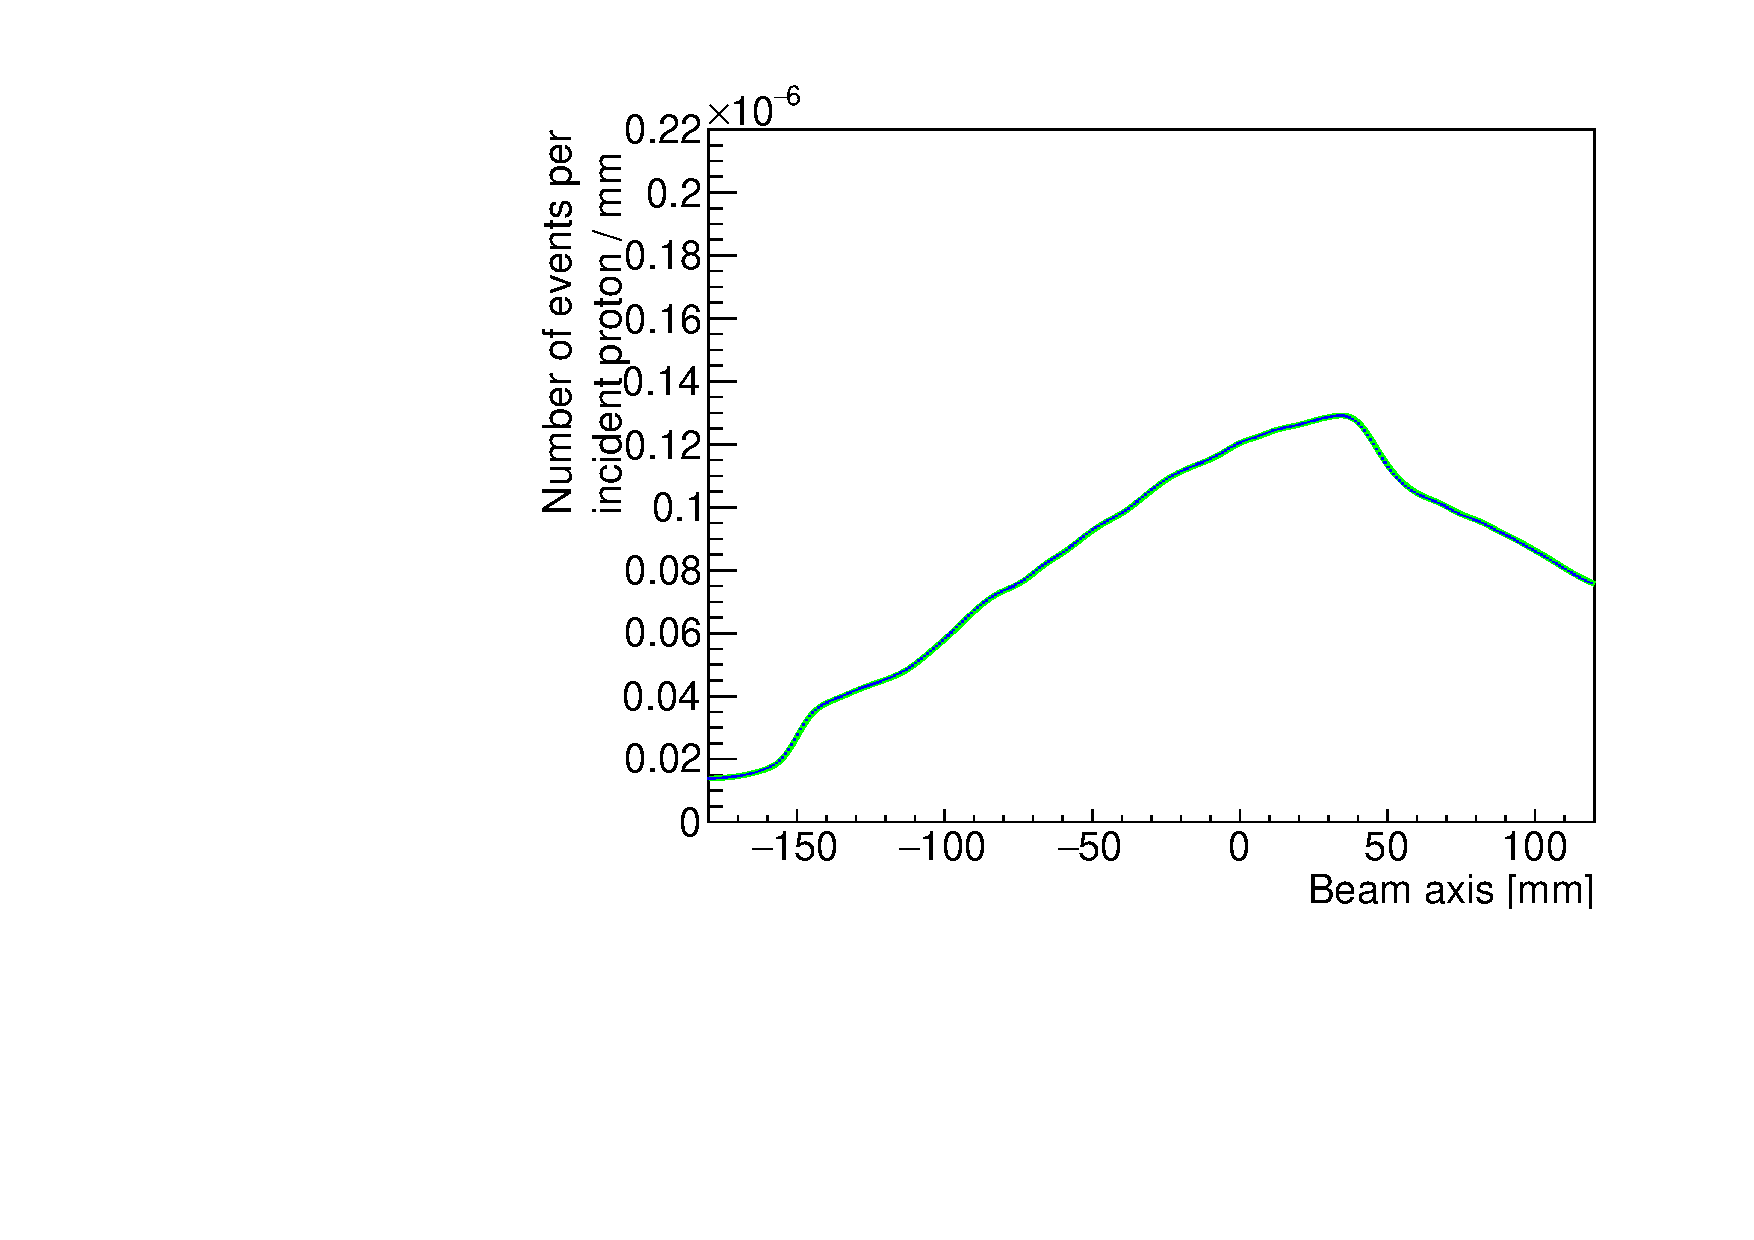
\includegraphics[width=0.48\textwidth]{./Figure/reference_LC.pdf}} 
\subfloat[\label{fig:fig_Results_Estimation_Camera_Profil_highStat_CC_simulation_Hadronth_MLEM}]{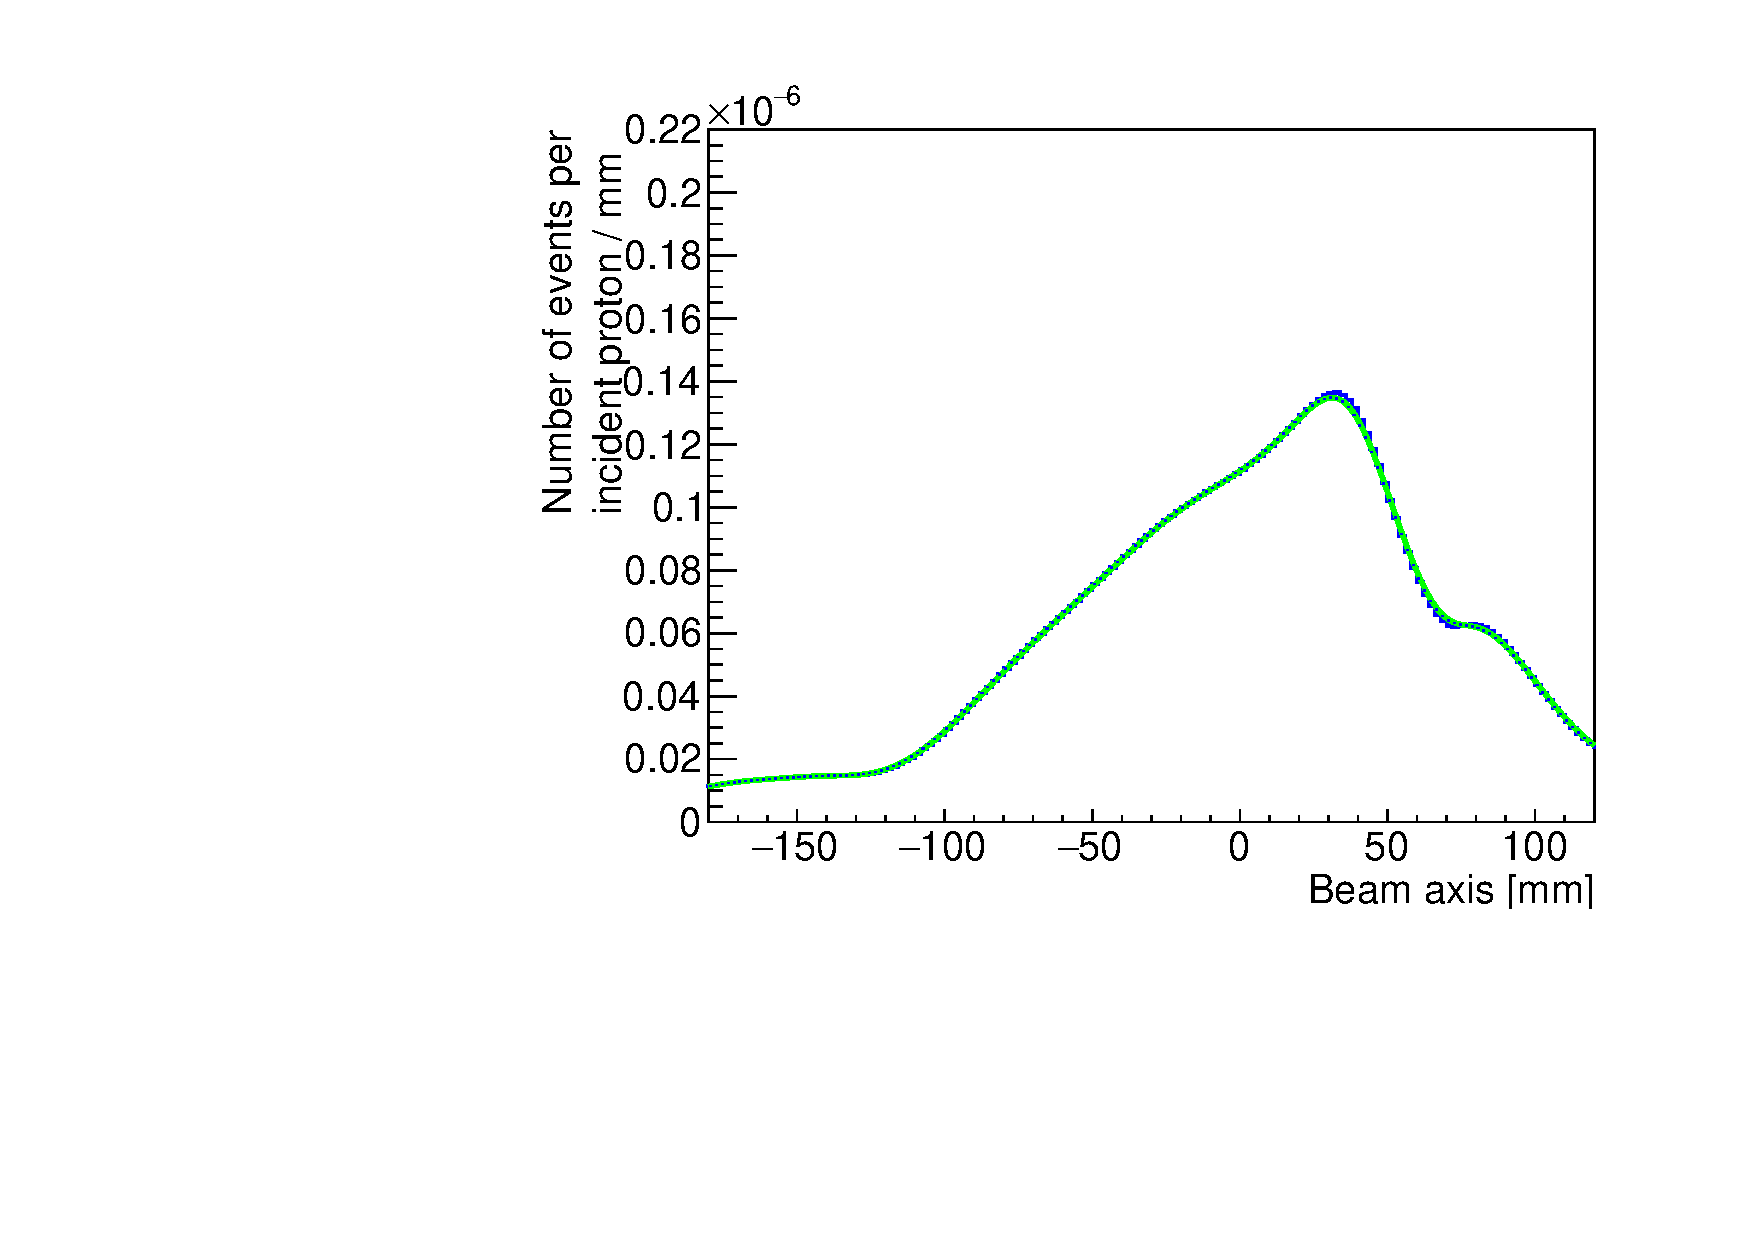
\includegraphics[width=0.48\textwidth]{./Figure/reference_MLEM_2it.pdf}}\\
%\subfloat[\label{fig:fig_Estimation_Camera_CC_NURBS_Poisson_LC}]{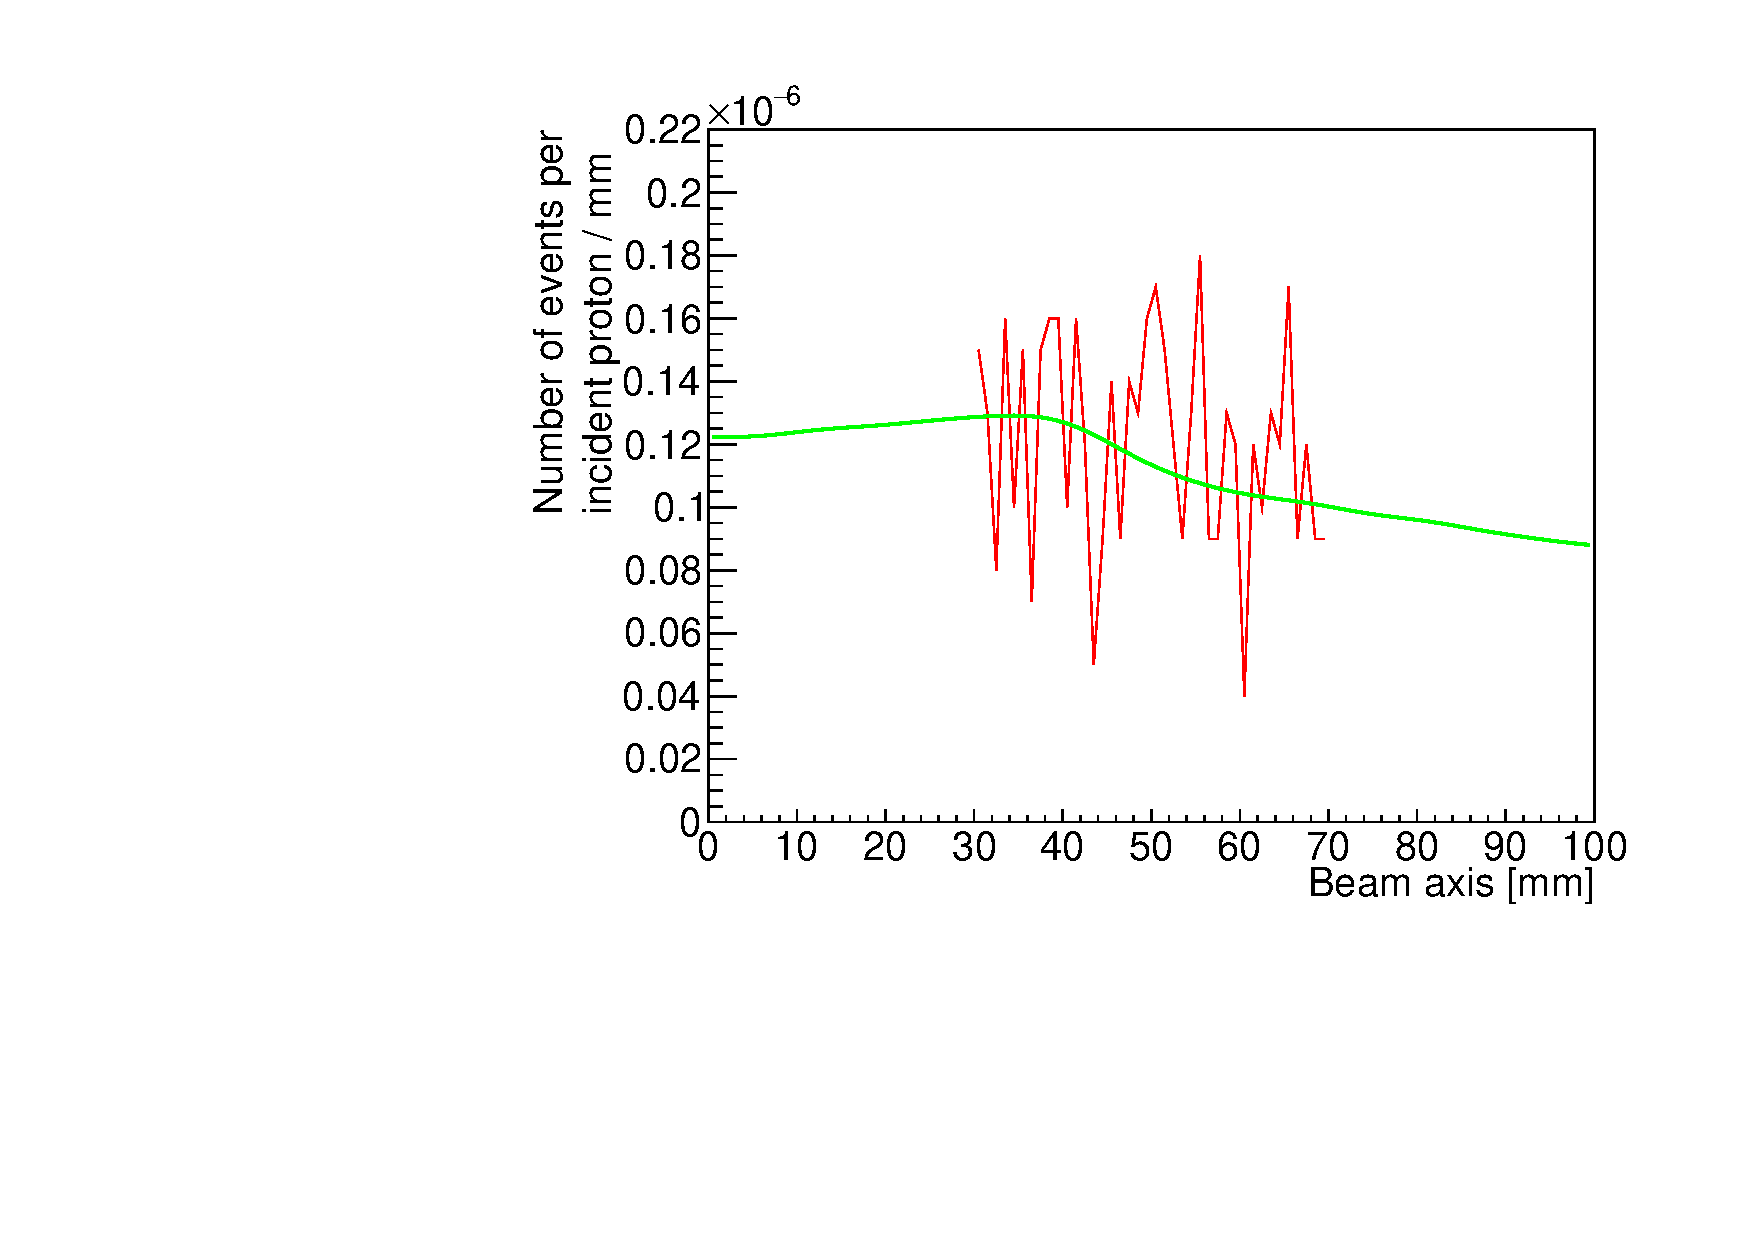
\includegraphics[width=0.48\textwidth]{./Figure/Results_forHadronthPaper/profile_Poisson_lineCone_green.pdf}}
\subfloat[\label{fig:fig_Estimation_Camera_CC_NURBS_Poisson_LC}]{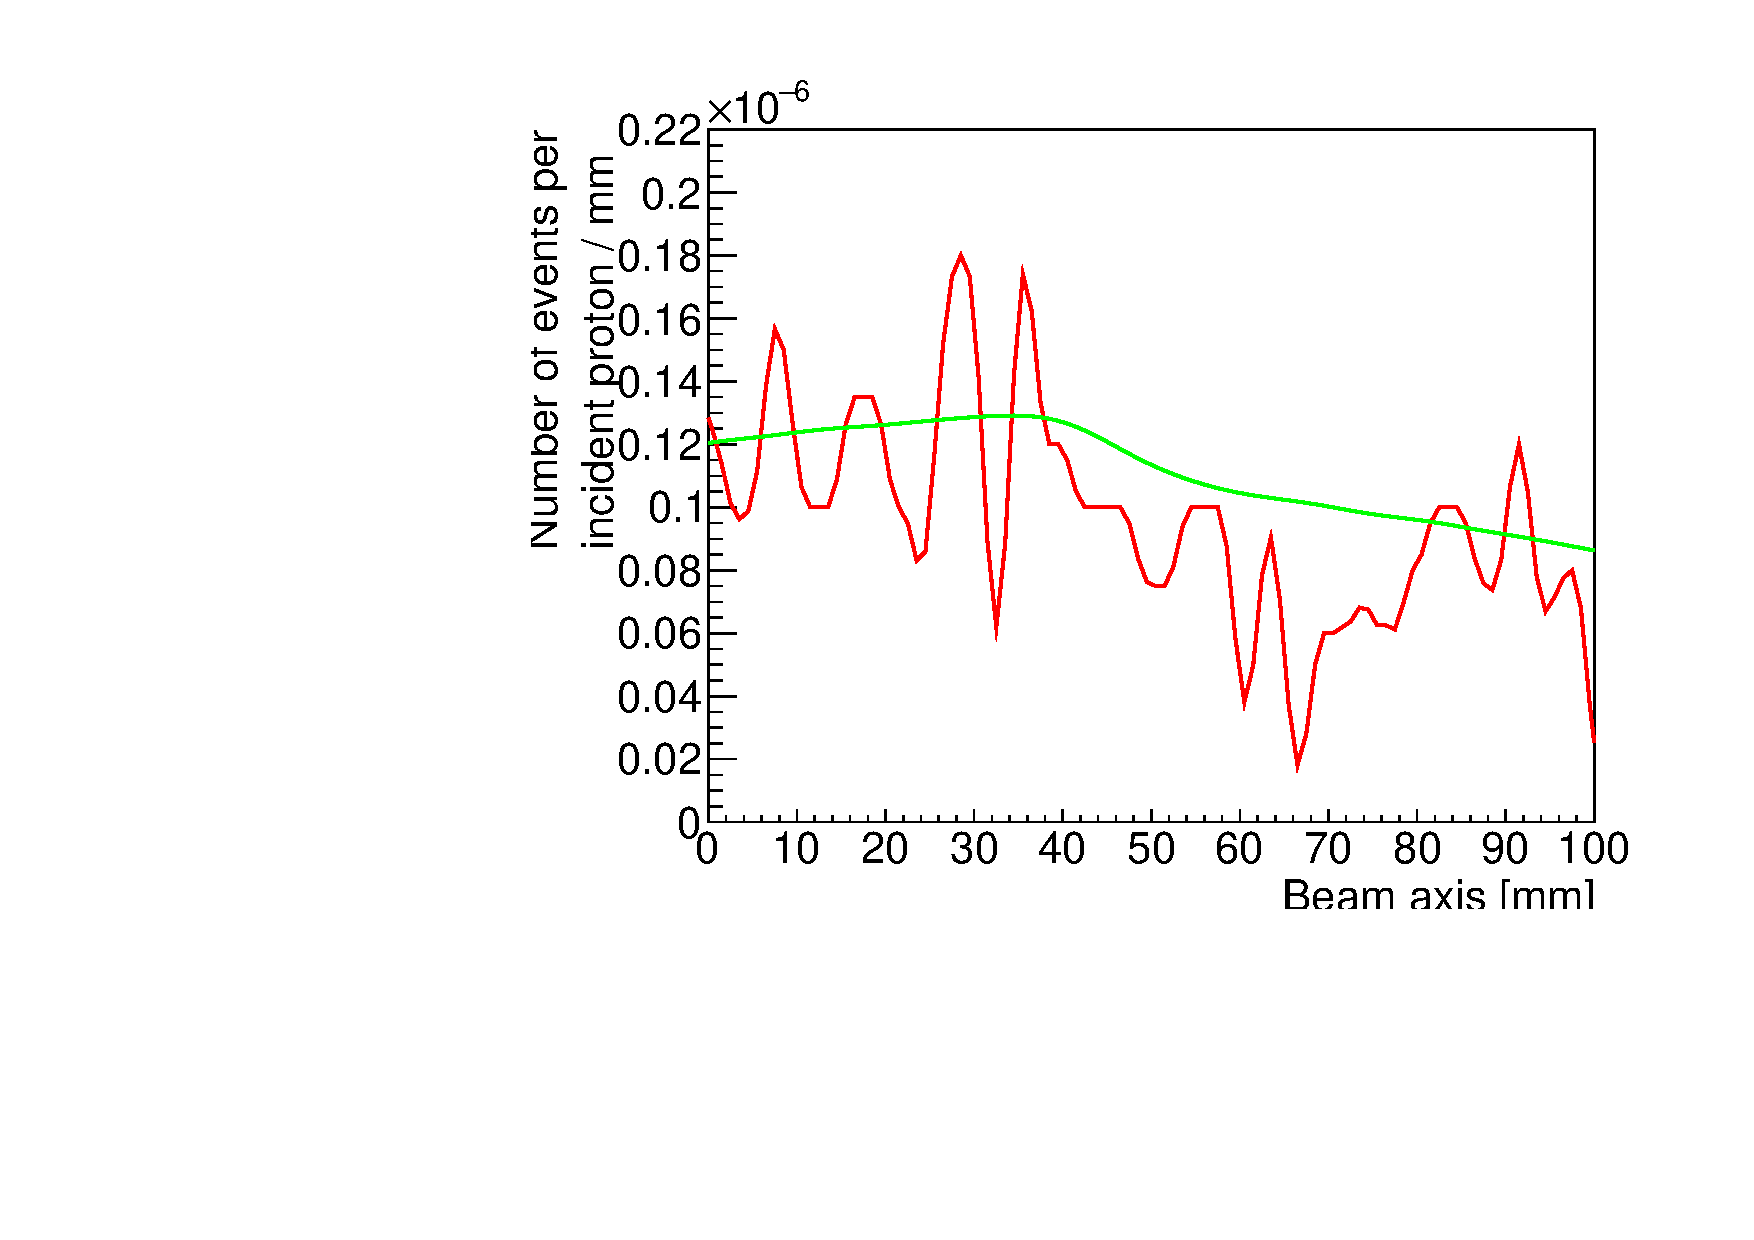
\includegraphics[width=0.48\textwidth]{./Figure/referenceVSlowstat_LC.pdf}}
\subfloat[\label{fig:fig_Estimation_Camera_CC_NURBS_Poisson_MLEM}]{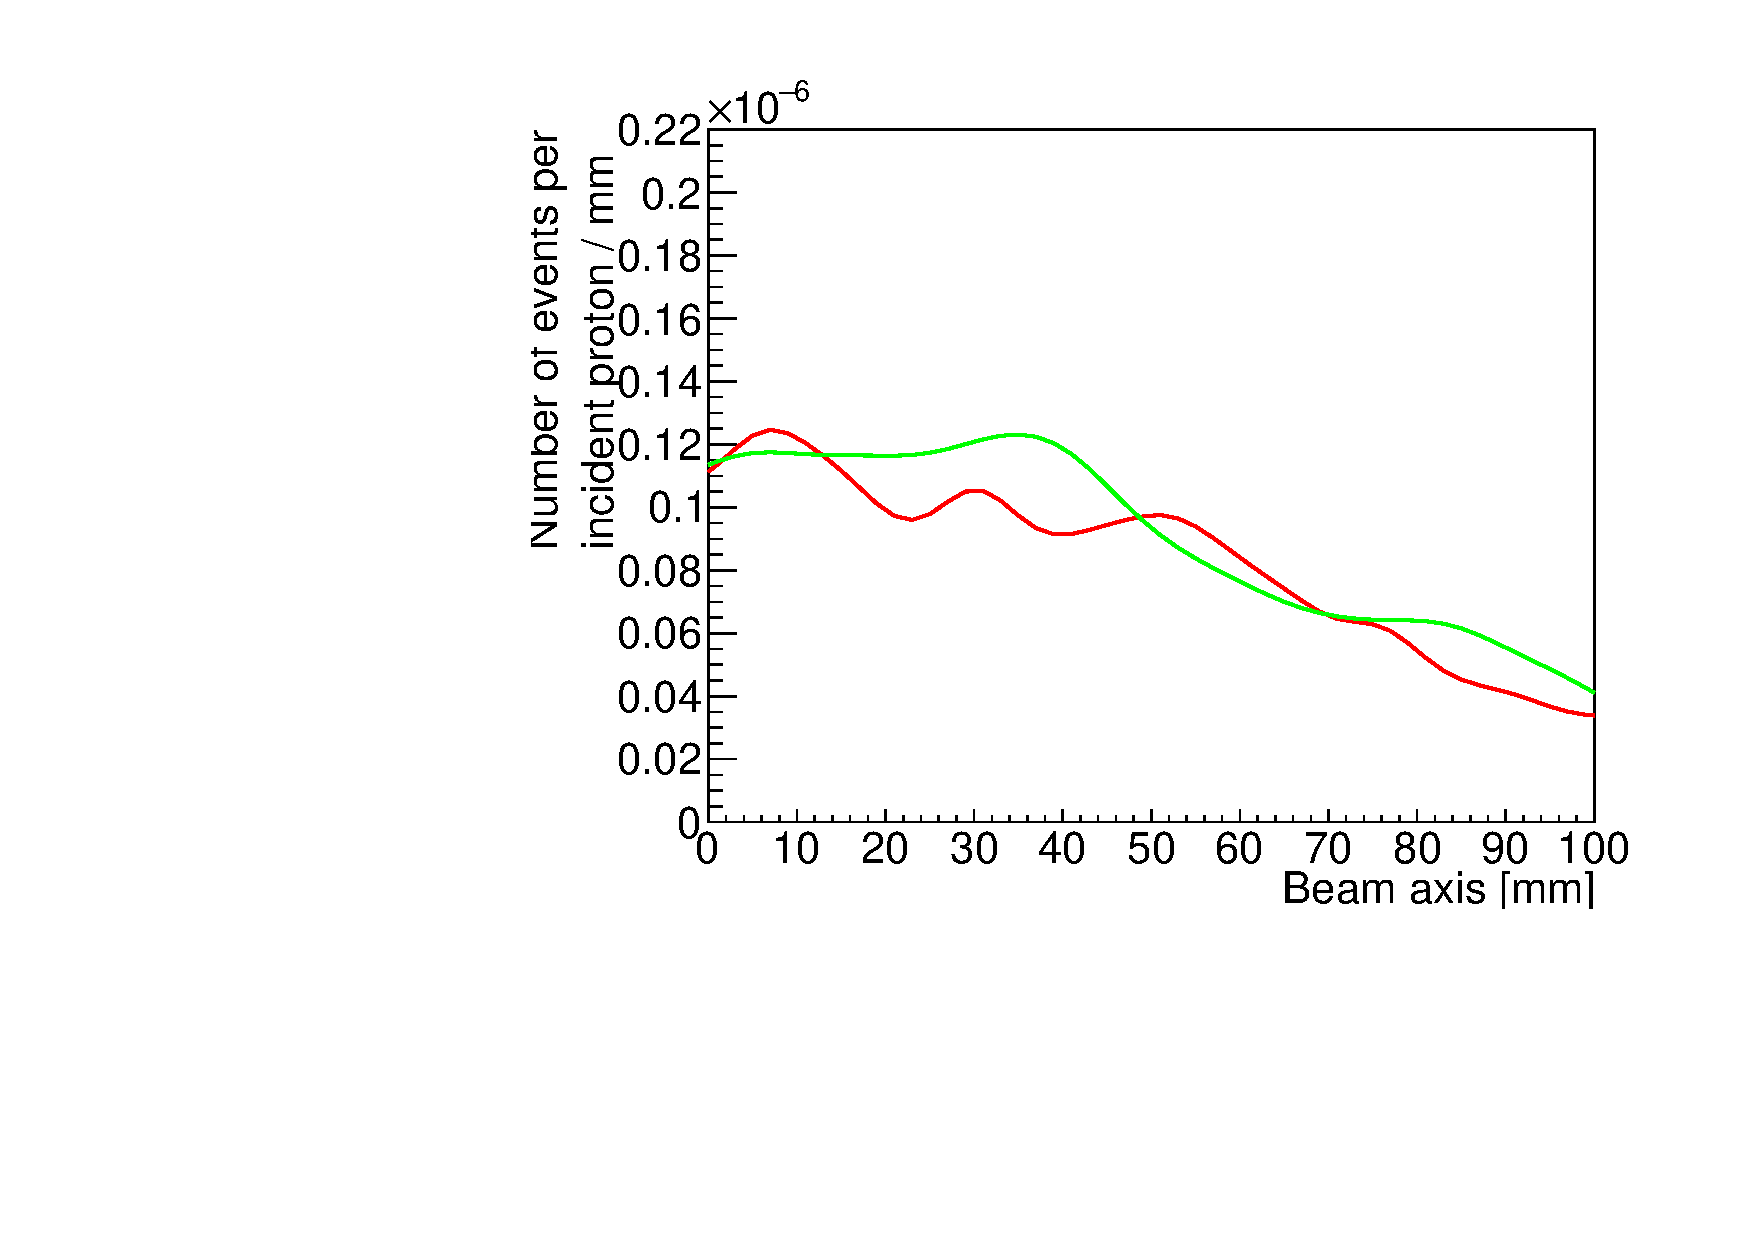
\includegraphics[width=0.48\textwidth]{./Figure/profiles_MLEM.pdf}}\\
\caption{Top row: line-cone (a) and LM-MLEM (b) reconstructed reference profile (blue histogram) for 2$\times10^{10}$ incident protons, at a beam intensity of 1 proton per bunch, with the NURBS related curves (green solid lines). Bottom row: NURBS curve (green) obtained after the normalization to a $10^8$ incident protons statistics, and Poisson generated statistical fluctuations (red) in the expected fall-off region, for the line-cone precision evaluation method (c), and profile realization for the LM-MLEM precision analysis (red -- d) obtained with the reconstruction of a data subset (for 10$^{8}$ incident protons) extracted from the reference profile data set.}
\end{figure}

\begin{figure}
  \centering
 % \subfloat[\label{fig:fig_Results_Precision_Distribution_Variation_CC_simulation_Hadronth_LC} ]{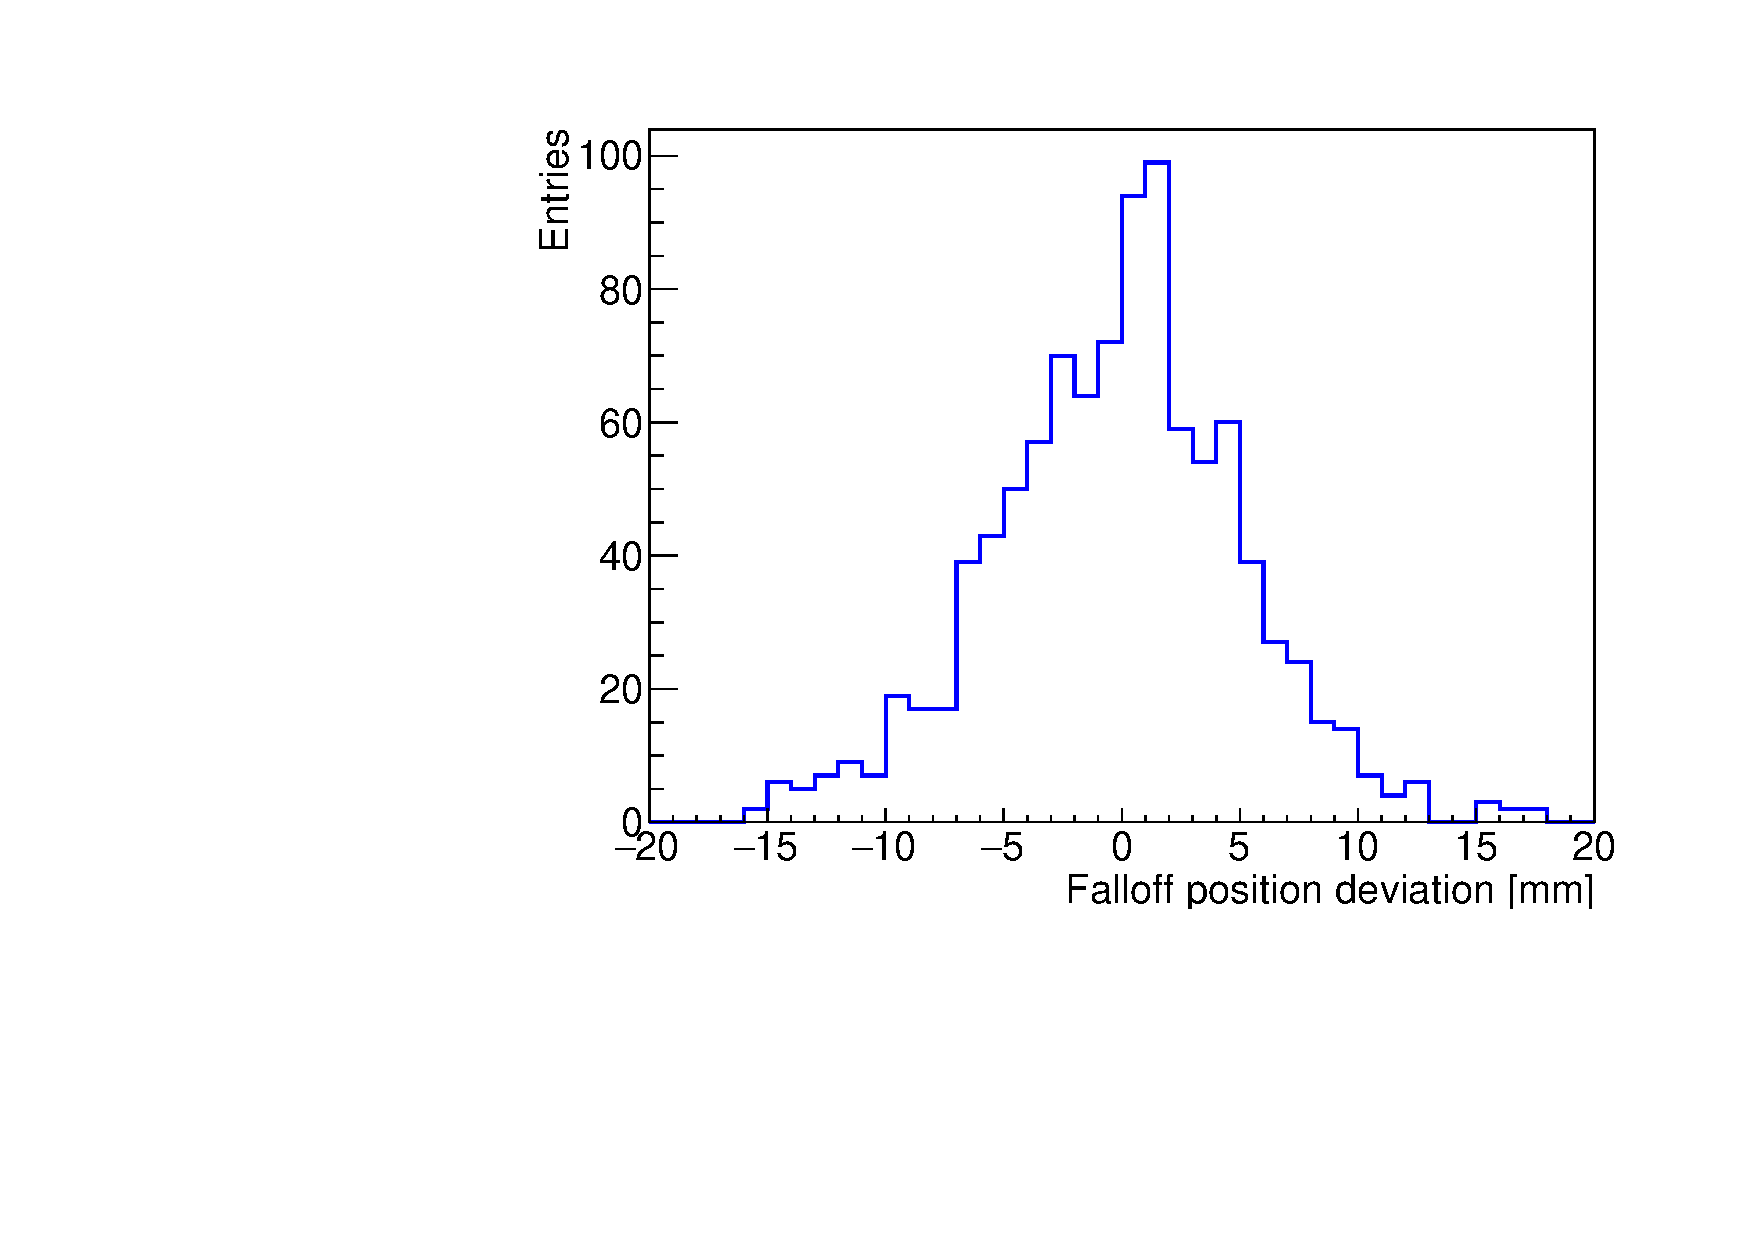
\includegraphics[width=0.48\textwidth, height = 5cm]{./Figure/new/LC_histo_deviations.pdf}}
 \subfloat[\label{fig:fig_Results_Precision_Distribution_Variation_CC_simulation_Hadronth_LC} ]{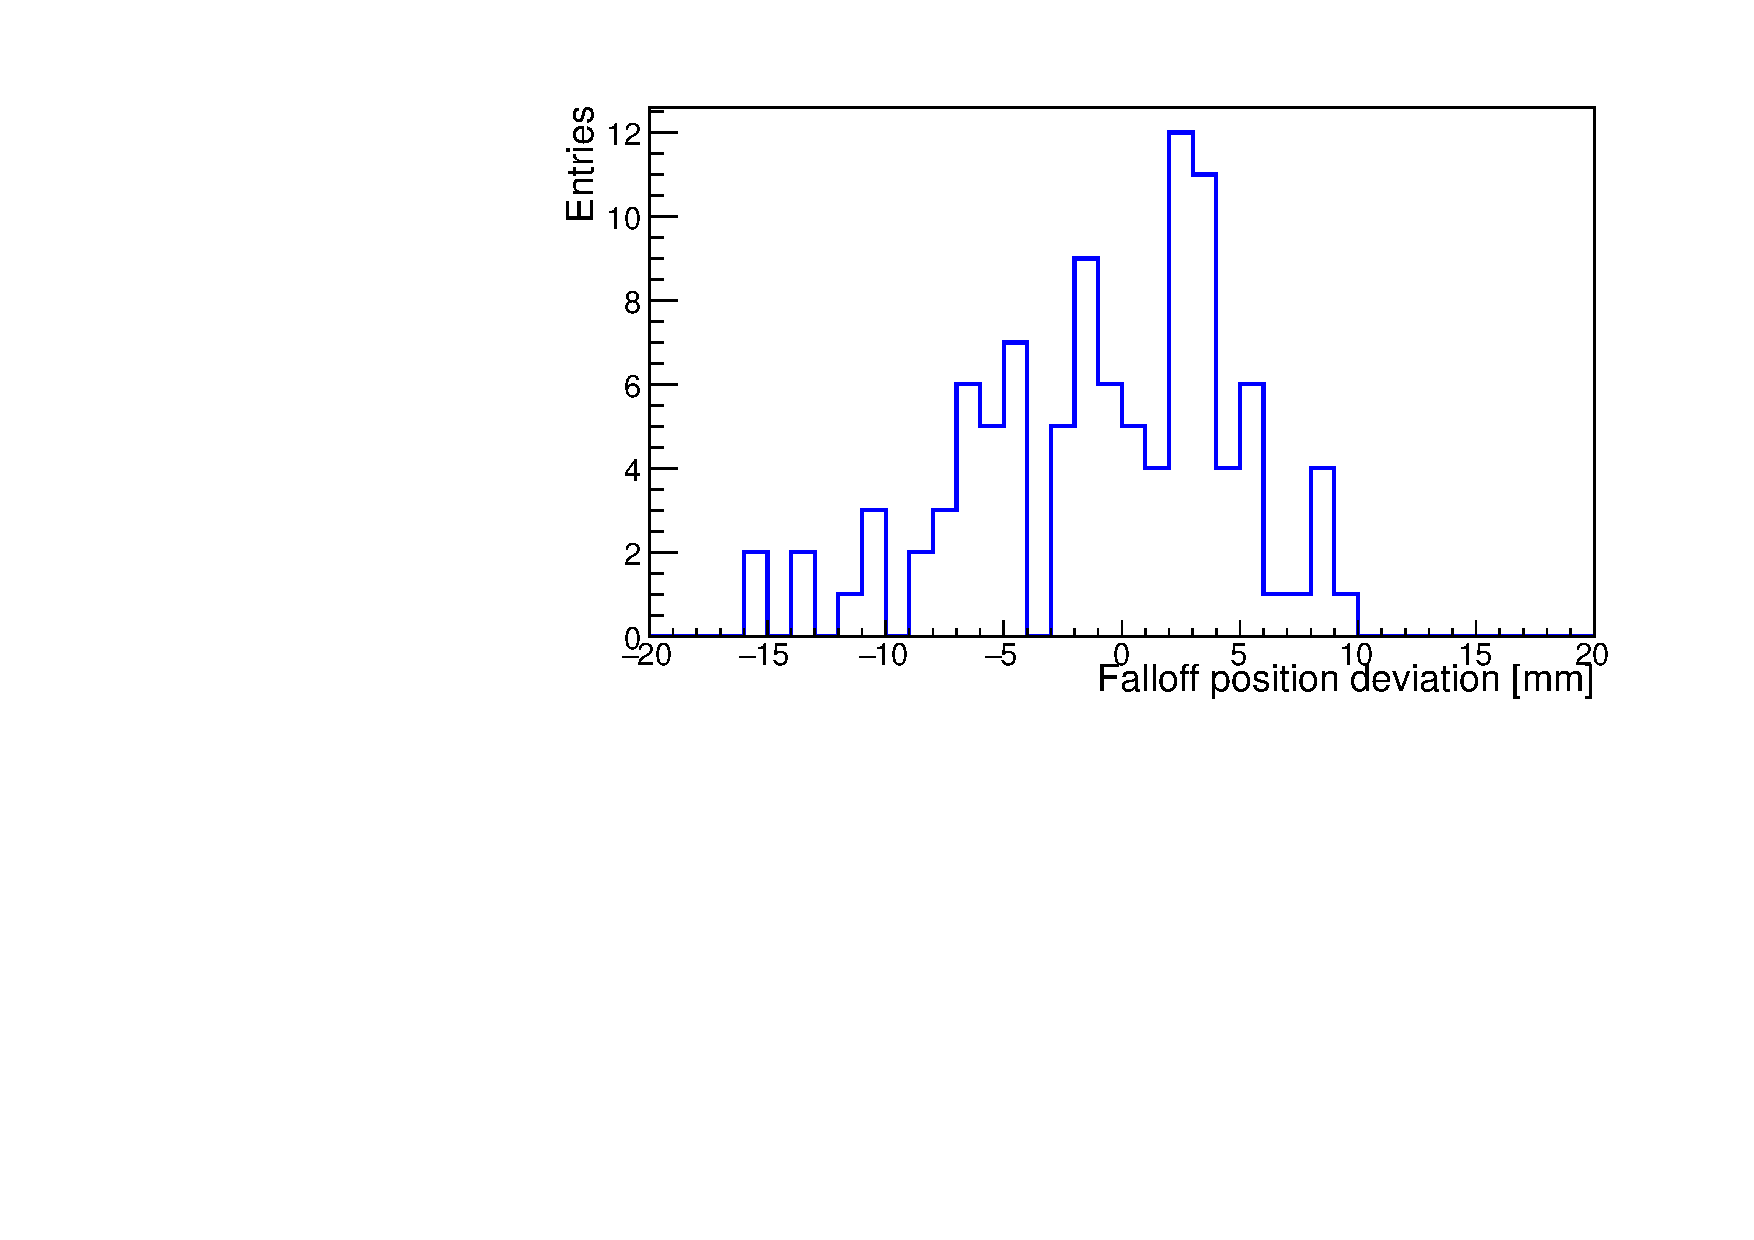
\includegraphics[width=0.48\textwidth, height = 5cm]{./Figure/deviations_LC.pdf}}  
  \subfloat[\label{fig:fig_Results_Precision_Distribution_Variation_CC_simulation_Hadronth_MLEM} ]{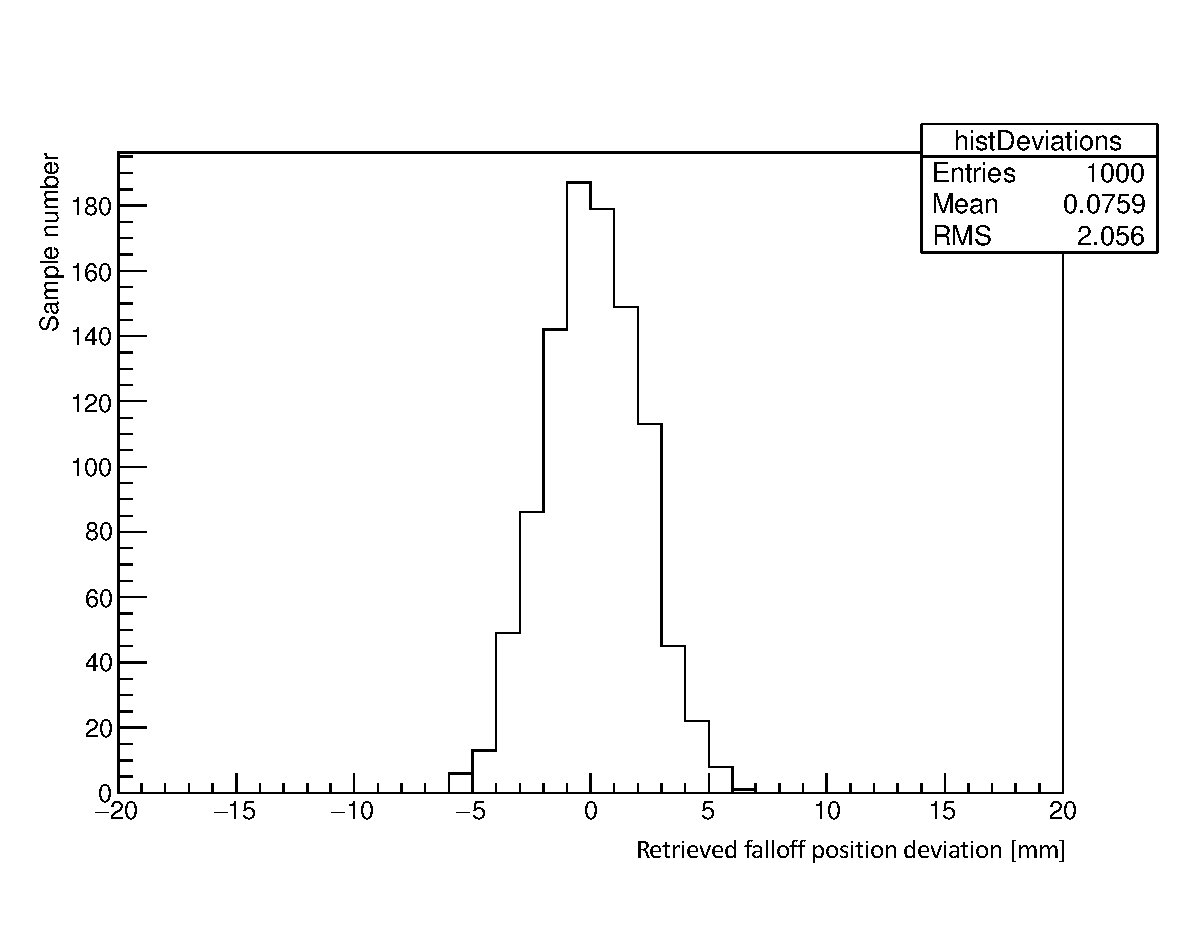
\includegraphics[width=0.48\textwidth, height = 5cm]{./Figure/deviation_MLEM.pdf}}
  \caption{Distributions of the fall-off position deviation with respect to the fall-off position of the high statistics reference profile for 1000 realizations with 10$^8$ primary protons obtained with line-cone reconstruction (left) and for 100 realizations with 10$^8$ primary protons obtained with the LM-MLEM reconstruction (right). The standard deviation of these distributions represents the Compton camera precision for the selected statistics.}
\end{figure}

The analysis method described in section~\ref{MatMeth:precision} is applied to the different PG obtained profiles to retrieve the camera precision in the fall-off identification. The results are shown in Figure~\ref{fig:precision}, where the two reconstruction methods are represented by different markers.

\begin{figure}	
\centering
%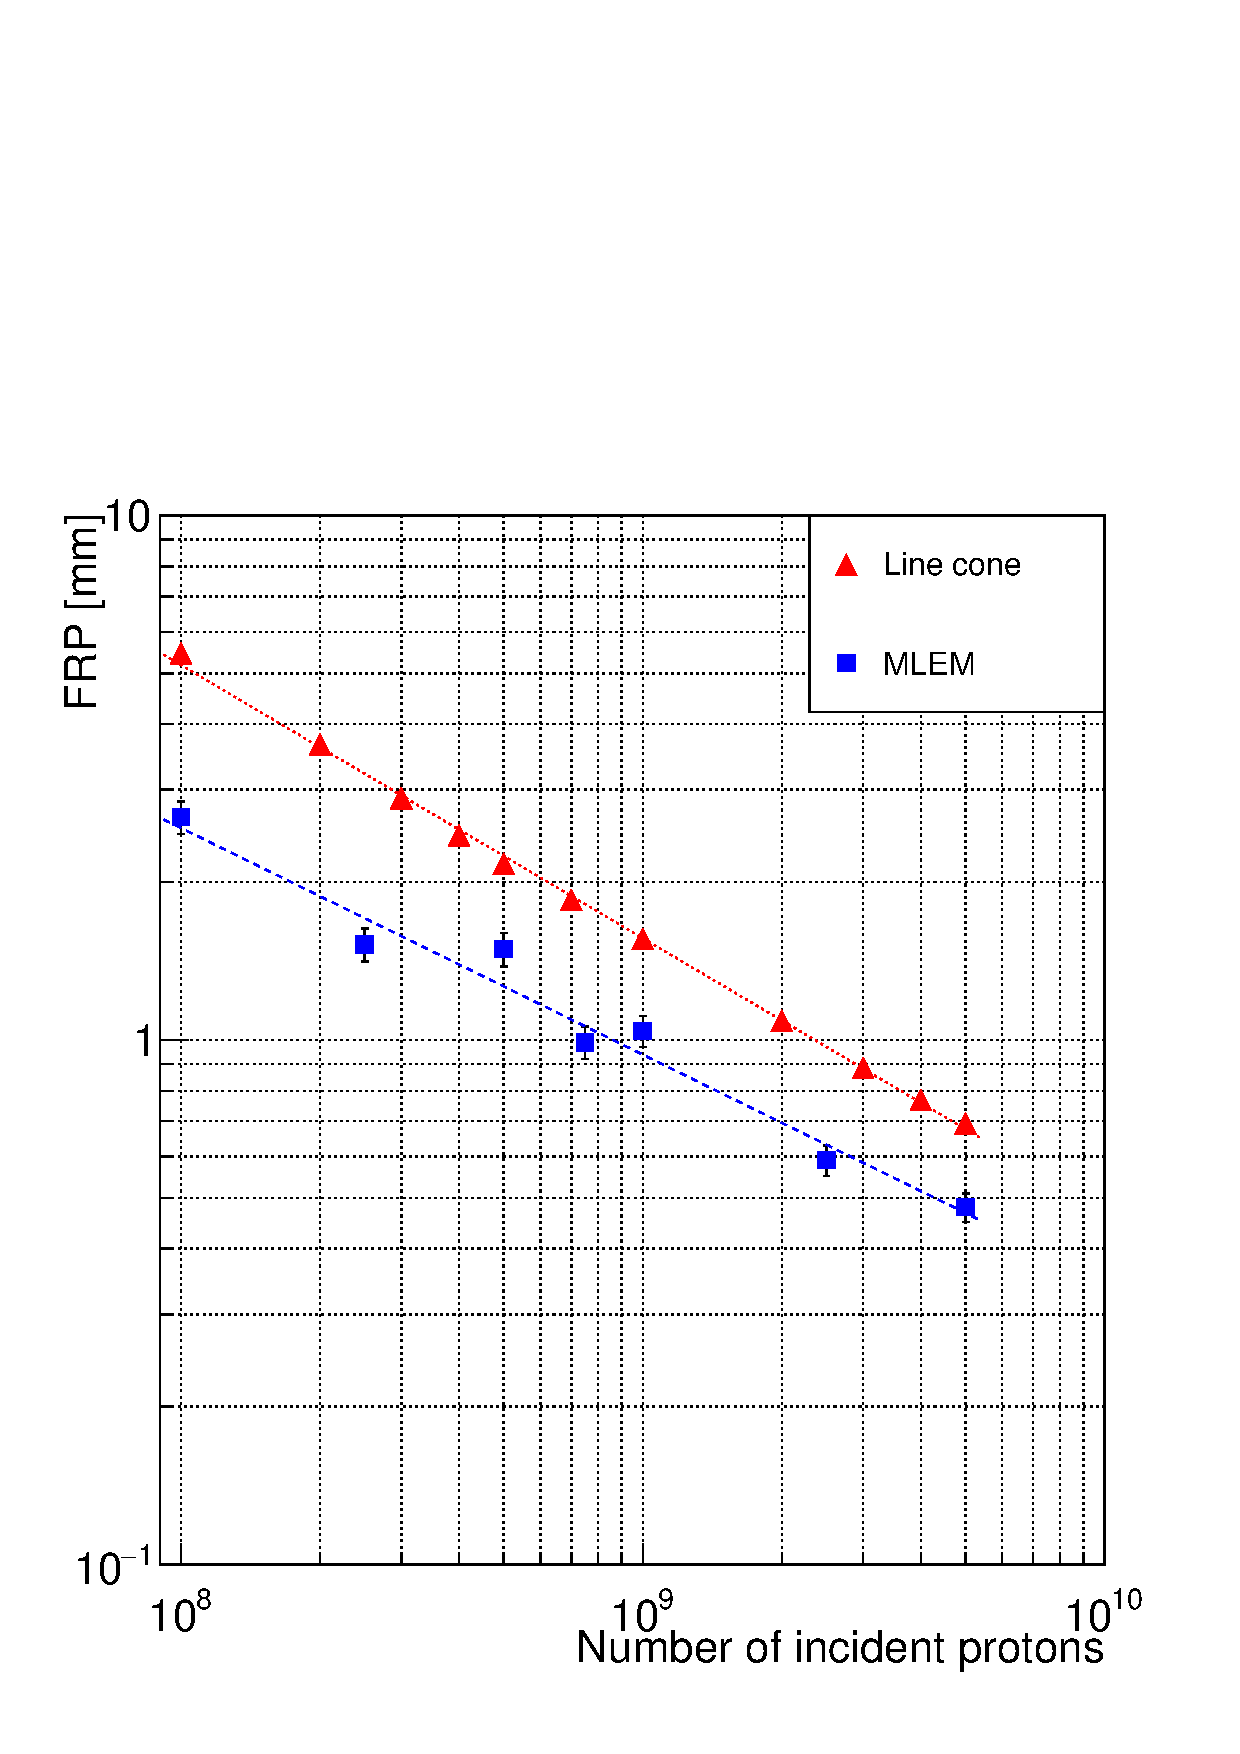
\includegraphics[width=0.6\textwidth]{./Figure/precision_2it.pdf}
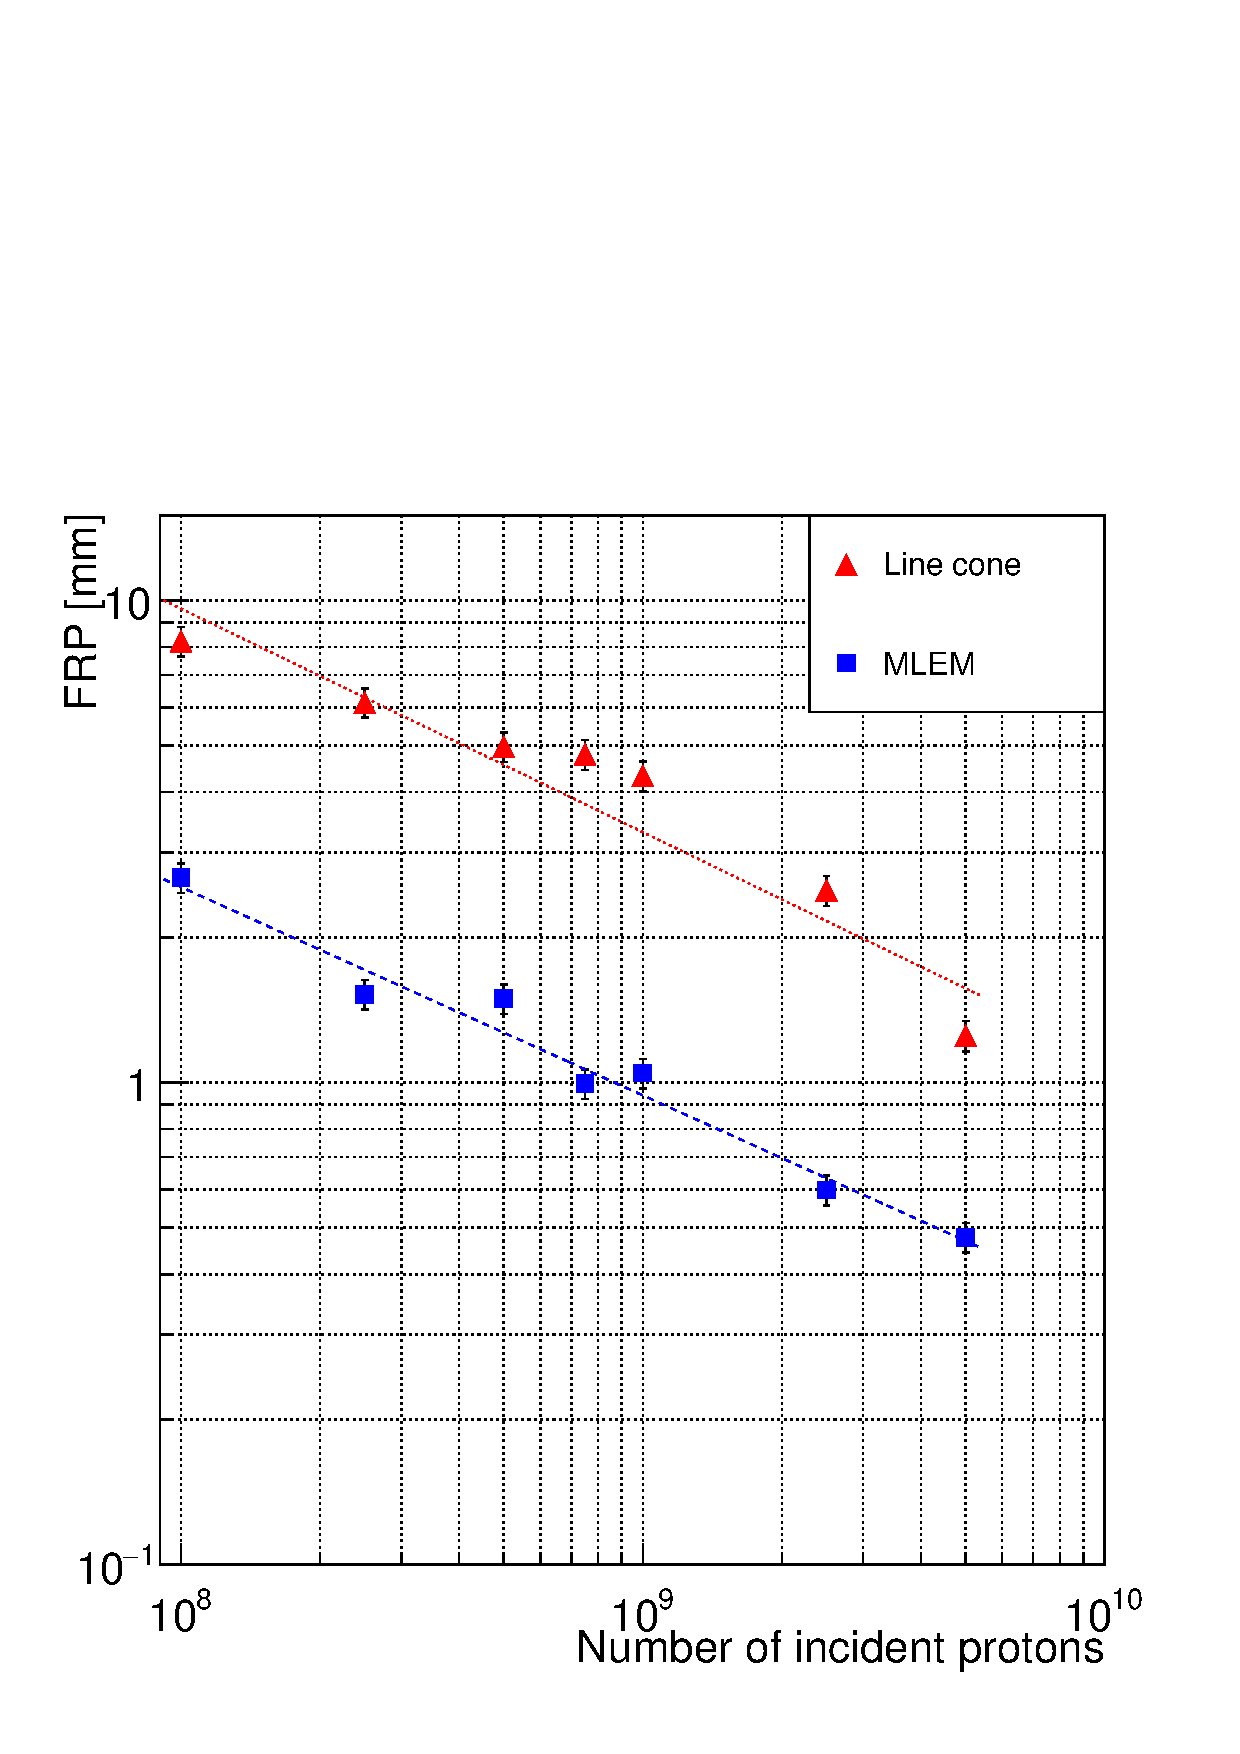
\includegraphics[width=0.6\textwidth]{./Figure/precision_LC_MLEM.pdf}
\caption{Fall-off retrieval precision (FRP) for two different reconstruction algorithms: line-cone and LM-MLEM. The precision is shown as a function of the total number of incident protons, in the range [$10^{8}$, $5\times10^{9}$].}	
\label{fig:precision}
\end{figure}

The iterative MLEM reconstruction method enables one to achieve a better precision with respect to the line-cone algorithm: the fall-off retrieval precision (FRP) is improved by a factor between 2.6 and 5 in the whole range of statistics explored. A linear behavior, highlighted by the performed linear fit of the two data sets, is verified with increasing number of primary protons, starting from the single spot scale of about 10$^8$ primaries, till $5\times10^9$ protons, which can correspond to the monitoring of a group of spots with the same planned range. 

